\documentclass[1p]{elsarticle_modified}
%\bibliographystyle{elsarticle-num}

%\usepackage[colorlinks]{hyperref}
%\usepackage{abbrmath_seonhwa} %\Abb, \Ascr, \Acal ,\Abf, \Afrak
\usepackage{amsfonts}
\usepackage{amssymb}
\usepackage{amsmath}
\usepackage{amsthm}
\usepackage{scalefnt}
\usepackage{amsbsy}
\usepackage{kotex}
\usepackage{caption}
\usepackage{subfig}
\usepackage{color}
\usepackage{graphicx}
\usepackage{xcolor} %% white, black, red, green, blue, cyan, magenta, yellow
\usepackage{float}
\usepackage{setspace}
\usepackage{hyperref}

\usepackage{tikz}
\usetikzlibrary{arrows}

\usepackage{multirow}
\usepackage{array} % fixed length table
\usepackage{hhline}

%%%%%%%%%%%%%%%%%%%%%
\makeatletter
\renewcommand*\env@matrix[1][\arraystretch]{%
	\edef\arraystretch{#1}%
	\hskip -\arraycolsep
	\let\@ifnextchar\new@ifnextchar
	\array{*\c@MaxMatrixCols c}}
\makeatother %https://tex.stackexchange.com/questions/14071/how-can-i-increase-the-line-spacing-in-a-matrix
%%%%%%%%%%%%%%%

\usepackage[normalem]{ulem}

\newcommand{\msout}[1]{\ifmmode\text{\sout{\ensuremath{#1}}}\else\sout{#1}\fi}
%SOURCE: \msout is \stkout macro in https://tex.stackexchange.com/questions/20609/strikeout-in-math-mode

\newcommand{\cancel}[1]{
	\ifmmode
	{\color{red}\msout{#1}}
	\else
	{\color{red}\sout{#1}}
	\fi
}

\newcommand{\add}[1]{
	{\color{blue}\uwave{#1}}
}

\newcommand{\replace}[2]{
	\ifmmode
	{\color{red}\msout{#1}}{\color{blue}\uwave{#2}}
	\else
	{\color{red}\sout{#1}}{\color{blue}\uwave{#2}}
	\fi
}

\newcommand{\Sol}{\mathcal{S}} %segment
\newcommand{\D}{D} %diagram
\newcommand{\A}{\mathcal{A}} %arc


%%%%%%%%%%%%%%%%%%%%%%%%%%%%%5 test

\def\sl{\operatorname{\textup{SL}}(2,\Cbb)}
\def\psl{\operatorname{\textup{PSL}}(2,\Cbb)}
\def\quan{\mkern 1mu \triangleright \mkern 1mu}

\theoremstyle{definition}
\newtheorem{thm}{Theorem}[section]
\newtheorem{prop}[thm]{Proposition}
\newtheorem{lem}[thm]{Lemma}
\newtheorem{ques}[thm]{Question}
\newtheorem{cor}[thm]{Corollary}
\newtheorem{defn}[thm]{Definition}
\newtheorem{exam}[thm]{Example}
\newtheorem{rmk}[thm]{Remark}
\newtheorem{alg}[thm]{Algorithm}

\newcommand{\I}{\sqrt{-1}}
\begin{document}

%\begin{frontmatter}
%
%\title{Boundary parabolic representations of knots up to 8 crossings}
%
%%% Group authors per affiliation:
%\author{Yunhi Cho} 
%\address{Department of Mathematics, University of Seoul, Seoul, Korea}
%\ead{yhcho@uos.ac.kr}
%
%
%\author{Seonhwa Kim} %\fnref{s_kim}}
%\address{Center for Geometry and Physics, Institute for Basic Science, Pohang, 37673, Korea}
%\ead{ryeona17@ibs.re.kr}
%
%\author{Hyuk Kim}
%\address{Department of Mathematical Sciences, Seoul National University, Seoul 08826, Korea}
%\ead{hyukkim@snu.ac.kr}
%
%\author{Seokbeom Yoon}
%\address{Department of Mathematical Sciences, Seoul National University, Seoul, 08826,  Korea}
%\ead{sbyoon15@snu.ac.kr}
%
%\begin{abstract}
%We find all boundary parabolic representation of knots up to 8 crossings.
%
%\end{abstract}
%\begin{keyword}
%    \MSC[2010] 57M25 
%\end{keyword}
%
%\end{frontmatter}

%\linenumbers
%\tableofcontents
%
\newcommand\colored[1]{\textcolor{white}{\rule[-0.35ex]{0.8em}{1.4ex}}\kern-0.8em\color{red} #1}%
%\newcommand\colored[1]{\textcolor{white}{ #1}\kern-2.17ex	\textcolor{white}{ #1}\kern-1.81ex	\textcolor{white}{ #1}\kern-2.15ex\color{red}#1	}

{\Large $\underline{12a_{0994}~(K12a_{0994})}$}

\setlength{\tabcolsep}{10pt}
\renewcommand{\arraystretch}{1.6}
\vspace{1cm}\begin{tabular}{m{100pt}>{\centering\arraybackslash}m{274pt}}
\multirow{5}{120pt}{
	\centering
	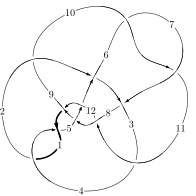
\includegraphics[width=112pt]{../../../GIT/diagram.site/Diagrams/png/1795_12a_0994.png}\\
\ \ \ A knot diagram\footnotemark}&
\allowdisplaybreaks
\textbf{Linearized knot diagam} \\
\cline{2-2}
 &
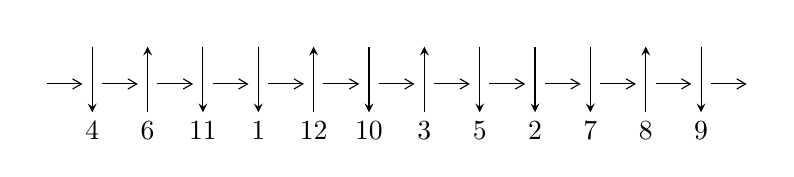
\begin{tikzpicture}[x=20pt, y=17pt]
	% nodes
	\node (C0) at (0, 0) {};
	\node (C1) at (1, 0) {};
	\node (C1U) at (1, +1) {};
	\node (C1D) at (1, -1) {4};

	\node (C2) at (2, 0) {};
	\node (C2U) at (2, +1) {};
	\node (C2D) at (2, -1) {6};

	\node (C3) at (3, 0) {};
	\node (C3U) at (3, +1) {};
	\node (C3D) at (3, -1) {11};

	\node (C4) at (4, 0) {};
	\node (C4U) at (4, +1) {};
	\node (C4D) at (4, -1) {1};

	\node (C5) at (5, 0) {};
	\node (C5U) at (5, +1) {};
	\node (C5D) at (5, -1) {12};

	\node (C6) at (6, 0) {};
	\node (C6U) at (6, +1) {};
	\node (C6D) at (6, -1) {10};

	\node (C7) at (7, 0) {};
	\node (C7U) at (7, +1) {};
	\node (C7D) at (7, -1) {3};

	\node (C8) at (8, 0) {};
	\node (C8U) at (8, +1) {};
	\node (C8D) at (8, -1) {5};

	\node (C9) at (9, 0) {};
	\node (C9U) at (9, +1) {};
	\node (C9D) at (9, -1) {2};

	\node (C10) at (10, 0) {};
	\node (C10U) at (10, +1) {};
	\node (C10D) at (10, -1) {7};

	\node (C11) at (11, 0) {};
	\node (C11U) at (11, +1) {};
	\node (C11D) at (11, -1) {8};

	\node (C12) at (12, 0) {};
	\node (C12U) at (12, +1) {};
	\node (C12D) at (12, -1) {9};
	\node (C13) at (13, 0) {};

	% arrows
	\draw[->,>={angle 60}]
	(C0) edge (C1) (C1) edge (C2) (C2) edge (C3) (C3) edge (C4) (C4) edge (C5) (C5) edge (C6) (C6) edge (C7) (C7) edge (C8) (C8) edge (C9) (C9) edge (C10) (C10) edge (C11) (C11) edge (C12) (C12) edge (C13) ;	\draw[->,>=stealth]
	(C1U) edge (C1D) (C2D) edge (C2U) (C3U) edge (C3D) (C4U) edge (C4D) (C5D) edge (C5U) (C6U) edge (C6D) (C7D) edge (C7U) (C8U) edge (C8D) (C9U) edge (C9D) (C10U) edge (C10D) (C11D) edge (C11U) (C12U) edge (C12D) ;
	\end{tikzpicture} \\
\hhline{~~} \\& 
\textbf{Solving Sequence} \\ \cline{2-2} 
 &
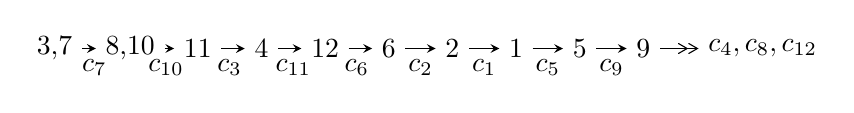
\begin{tikzpicture}[x=23pt, y=7pt]
	% node
	\node (A0) at (-1/8, 0) {3,7};
	\node (A1) at (17/16, 0) {8,10};
	\node (A2) at (17/8, 0) {11};
	\node (A3) at (25/8, 0) {4};
	\node (A4) at (33/8, 0) {12};
	\node (A5) at (41/8, 0) {6};
	\node (A6) at (49/8, 0) {2};
	\node (A7) at (57/8, 0) {1};
	\node (A8) at (65/8, 0) {5};
	\node (A9) at (73/8, 0) {9};
	\node (C1) at (1/2, -1) {$c_{7}$};
	\node (C2) at (13/8, -1) {$c_{10}$};
	\node (C3) at (21/8, -1) {$c_{3}$};
	\node (C4) at (29/8, -1) {$c_{11}$};
	\node (C5) at (37/8, -1) {$c_{6}$};
	\node (C6) at (45/8, -1) {$c_{2}$};
	\node (C7) at (53/8, -1) {$c_{1}$};
	\node (C8) at (61/8, -1) {$c_{5}$};
	\node (C9) at (69/8, -1) {$c_{9}$};
	\node (A10) at (11, 0) {$c_{4},c_{8},c_{12}$};

	% edge
	\draw[->,>=stealth]	
	(A0) edge (A1) (A1) edge (A2) (A2) edge (A3) (A3) edge (A4) (A4) edge (A5) (A5) edge (A6) (A6) edge (A7) (A7) edge (A8) (A8) edge (A9) ;
	\draw[->>,>={angle 60}]	
	(A9) edge (A10);
\end{tikzpicture} \\ 

\end{tabular} \\

\footnotetext{
The image of knot diagram is generated by the software ``\textbf{Draw programme}" developed by Andrew Bartholomew(\url{http://www.layer8.co.uk/maths/draw/index.htm\#Running-draw}), where we modified some parts for our purpose(\url{https://github.com/CATsTAILs/LinksPainter}).
}\phantom \\ \newline 
\centering \textbf{Ideals for irreducible components\footnotemark of $X_{\text{par}}$} 
 
\begin{align*}
I^u_{1}&=\langle 
1.33817\times10^{1959} u^{183}-1.96405\times10^{1958} u^{182}+\cdots+2.02336\times10^{1961} b+2.47768\times10^{1961},\\
\phantom{I^u_{1}}&\phantom{= \langle  }-8.13478\times10^{1960} u^{183}-1.70818\times10^{1961} u^{182}+\cdots+2.02336\times10^{1961} a+5.65089\times10^{1961},\\
\phantom{I^u_{1}}&\phantom{= \langle  }u^{184}+2 u^{183}+\cdots-32 u-8\rangle \\
I^u_{2}&=\langle 
-4.93935\times10^{75} u^{40}-8.59978\times10^{75} u^{39}+\cdots+4.56856\times10^{76} b+4.79524\times10^{76},\\
\phantom{I^u_{2}}&\phantom{= \langle  }-3.27638\times10^{75} u^{40}-7.74862\times10^{75} u^{39}+\cdots+4.56856\times10^{76} a-3.80076\times10^{76},\;u^{41}+u^{40}+\cdots-4 u+1\rangle \\
\\
\end{align*}
\raggedright * 2 irreducible components of $\dim_{\mathbb{C}}=0$, with total 225 representations.\\
\footnotetext{All coefficients of polynomials are rational numbers. But the coefficients are sometimes approximated in decimal forms when there is not enough margin.}
\newpage
\renewcommand{\arraystretch}{1}
\centering \section*{I. $I^u_{1}= \langle 1.34\times10^{1959} u^{183}-1.96\times10^{1958} u^{182}+\cdots+2.02\times10^{1961} b+2.48\times10^{1961},\;-8.13\times10^{1960} u^{183}-1.71\times10^{1961} u^{182}+\cdots+2.02\times10^{1961} a+5.65\times10^{1961},\;u^{184}+2 u^{183}+\cdots-32 u-8 \rangle$}
\flushleft \textbf{(i) Arc colorings}\\
\begin{tabular}{m{7pt} m{180pt} m{7pt} m{180pt} }
\flushright $a_{3}=$&$\begin{pmatrix}0\\u\end{pmatrix}$ \\
\flushright $a_{7}=$&$\begin{pmatrix}1\\0\end{pmatrix}$ \\
\flushright $a_{8}=$&$\begin{pmatrix}1\\- u^2\end{pmatrix}$ \\
\flushright $a_{10}=$&$\begin{pmatrix}0.402044 u^{183}+0.844233 u^{182}+\cdots-58.9819 u-2.79283\\-0.00661362 u^{183}+0.000970690 u^{182}+\cdots-10.3979 u-1.22454\end{pmatrix}$ \\
\flushright $a_{11}=$&$\begin{pmatrix}0.408658 u^{183}+0.843262 u^{182}+\cdots-48.5839 u-1.56829\\-0.00661362 u^{183}+0.000970690 u^{182}+\cdots-10.3979 u-1.22454\end{pmatrix}$ \\
\flushright $a_{4}=$&$\begin{pmatrix}0.909896 u^{183}+1.64149 u^{182}+\cdots+37.2159 u+22.6886\\0.0281559 u^{183}+0.0967861 u^{182}+\cdots-29.2844 u-4.80104\end{pmatrix}$ \\
\flushright $a_{12}=$&$\begin{pmatrix}0.376358 u^{183}+0.787522 u^{182}+\cdots-54.8823 u-2.58526\\-0.00972317 u^{183}-0.00502116 u^{182}+\cdots-10.4230 u-1.29541\end{pmatrix}$ \\
\flushright $a_{6}=$&$\begin{pmatrix}-0.606016 u^{183}-1.21272 u^{182}+\cdots+43.5390 u-6.41960\\-0.00588665 u^{183}-0.0406161 u^{182}+\cdots+25.4824 u+3.66070\end{pmatrix}$ \\
\flushright $a_{2}=$&$\begin{pmatrix}0.679492 u^{183}+1.20486 u^{182}+\cdots+85.5928 u+29.0130\\0.0772370 u^{183}+0.214338 u^{182}+\cdots-56.0102 u-7.17148\end{pmatrix}$ \\
\flushright $a_{1}=$&$\begin{pmatrix}0.691163 u^{183}+1.45581 u^{182}+\cdots-107.276 u-9.74903\\-0.0285364 u^{183}-0.0493336 u^{182}+\cdots-1.23104 u-1.31987\end{pmatrix}$ \\
\flushright $a_{5}=$&$\begin{pmatrix}0.240499 u^{183}+0.501494 u^{182}+\cdots-91.1375 u-10.7023\\-0.134023 u^{183}-0.272513 u^{182}+\cdots+10.9558 u-1.47174\end{pmatrix}$ \\
\flushright $a_{9}=$&$\begin{pmatrix}-0.196908 u^{183}-0.429208 u^{182}+\cdots+84.6171 u+10.1386\\0.106995 u^{183}+0.213012 u^{182}+\cdots-0.961589 u+1.44937\end{pmatrix}$\\&\end{tabular}
\flushleft \textbf{(ii) Obstruction class $= -1$}\\~\\
\flushleft \textbf{(iii) Cusp Shapes $= -0.577315 u^{183}-1.24671 u^{182}+\cdots+169.482 u+12.5623$}\\~\\
\newpage\renewcommand{\arraystretch}{1}
\flushleft \textbf{(iv) u-Polynomials at the component}\newline \\
\begin{tabular}{m{50pt}|m{274pt}}
Crossings & \hspace{64pt}u-Polynomials at each crossing \\
\hline $$\begin{aligned}c_{1},c_{4}\end{aligned}$$&$\begin{aligned}
&u^{184}+9 u^{183}+\cdots+7757548 u+603055
\end{aligned}$\\
\hline $$\begin{aligned}c_{2}\end{aligned}$$&$\begin{aligned}
&u^{184}-5 u^{183}+\cdots-76590 u-11783
\end{aligned}$\\
\hline $$\begin{aligned}c_{3}\end{aligned}$$&$\begin{aligned}
&u^{184}-2 u^{183}+\cdots-56849 u-15319
\end{aligned}$\\
\hline $$\begin{aligned}c_{5}\end{aligned}$$&$\begin{aligned}
&u^{184}+6 u^{183}+\cdots+50 u+1
\end{aligned}$\\
\hline $$\begin{aligned}c_{6},c_{10}\end{aligned}$$&$\begin{aligned}
&u^{184}- u^{183}+\cdots+4833 u+181
\end{aligned}$\\
\hline $$\begin{aligned}c_{7}\end{aligned}$$&$\begin{aligned}
&u^{184}-2 u^{183}+\cdots+32 u-8
\end{aligned}$\\
\hline $$\begin{aligned}c_{8}\end{aligned}$$&$\begin{aligned}
&u^{184}+10 u^{183}+\cdots+1097072 u+93376
\end{aligned}$\\
\hline $$\begin{aligned}c_{9}\end{aligned}$$&$\begin{aligned}
&u^{184}-3 u^{183}+\cdots+65011712 u-164626432
\end{aligned}$\\
\hline $$\begin{aligned}c_{11}\end{aligned}$$&$\begin{aligned}
&u^{184}+3 u^{183}+\cdots+2982702 u-149351
\end{aligned}$\\
\hline $$\begin{aligned}c_{12}\end{aligned}$$&$\begin{aligned}
&u^{184}+8 u^{183}+\cdots+5 u-7
\end{aligned}$\\
\hline
\end{tabular}\\~\\
\newpage\renewcommand{\arraystretch}{1}
\flushleft \textbf{(v) Riley Polynomials at the component}\newline \\
\begin{tabular}{m{50pt}|m{274pt}}
Crossings & \hspace{64pt}Riley Polynomials at each crossing \\
\hline $$\begin{aligned}c_{1},c_{4}\end{aligned}$$&$\begin{aligned}
&y^{184}+133 y^{183}+\cdots+18491955281616 y+363675333025
\end{aligned}$\\
\hline $$\begin{aligned}c_{2}\end{aligned}$$&$\begin{aligned}
&y^{184}+45 y^{183}+\cdots-4030990812 y+138839089
\end{aligned}$\\
\hline $$\begin{aligned}c_{3}\end{aligned}$$&$\begin{aligned}
&y^{184}-14 y^{183}+\cdots-14728626387 y+234671761
\end{aligned}$\\
\hline $$\begin{aligned}c_{5}\end{aligned}$$&$\begin{aligned}
&y^{184}+10 y^{183}+\cdots+8 y+1
\end{aligned}$\\
\hline $$\begin{aligned}c_{6},c_{10}\end{aligned}$$&$\begin{aligned}
&y^{184}-135 y^{183}+\cdots-656145 y+32761
\end{aligned}$\\
\hline $$\begin{aligned}c_{7}\end{aligned}$$&$\begin{aligned}
&y^{184}+16 y^{183}+\cdots+5856 y+64
\end{aligned}$\\
\hline $$\begin{aligned}c_{8}\end{aligned}$$&$\begin{aligned}
&y^{184}+60 y^{183}+\cdots+215273876736 y+8719077376
\end{aligned}$\\
\hline $$\begin{aligned}c_{9}\end{aligned}$$&$\begin{aligned}
&y^{184}-59 y^{183}+\cdots-2337403390977376256 y+27101862113050624
\end{aligned}$\\
\hline $$\begin{aligned}c_{11}\end{aligned}$$&$\begin{aligned}
&y^{184}-57 y^{183}+\cdots-4254754725390 y+22305721201
\end{aligned}$\\
\hline $$\begin{aligned}c_{12}\end{aligned}$$&$\begin{aligned}
&y^{184}+36 y^{183}+\cdots+8655 y+49
\end{aligned}$\\
\hline
\end{tabular}\\~\\
\newpage\flushleft \textbf{(vi) Complex Volumes and Cusp Shapes}
$$\begin{array}{c|c|c}  
\text{Solutions to }I^u_{1}& \I (\text{vol} + \sqrt{-1}CS) & \text{Cusp shape}\\
 \hline 
\begin{aligned}
u &= -0.398532 + 0.916383 I \\
a &= \phantom{-}0.785014 - 0.120928 I \\
b &= \phantom{-}0.557623 + 0.673511 I\end{aligned}
 & -0.23680 - 1.56240 I & \phantom{-0.000000 } 0 \\ \hline\begin{aligned}
u &= -0.398532 - 0.916383 I \\
a &= \phantom{-}0.785014 + 0.120928 I \\
b &= \phantom{-}0.557623 - 0.673511 I\end{aligned}
 & -0.23680 + 1.56240 I & \phantom{-0.000000 } 0 \\ \hline\begin{aligned}
u &= \phantom{-}0.897408 + 0.459546 I \\
a &= -0.627805 + 0.309171 I \\
b &= -0.412591 - 0.769997 I\end{aligned}
 & \phantom{-}5.82894 + 1.42303 I & \phantom{-0.000000 } 0 \\ \hline\begin{aligned}
u &= \phantom{-}0.897408 - 0.459546 I \\
a &= -0.627805 - 0.309171 I \\
b &= -0.412591 + 0.769997 I\end{aligned}
 & \phantom{-}5.82894 - 1.42303 I & \phantom{-0.000000 } 0 \\ \hline\begin{aligned}
u &= \phantom{-}0.298894 + 0.984405 I \\
a &= \phantom{-}1.031340 + 0.101557 I \\
b &= \phantom{-}1.31351 - 0.60603 I\end{aligned}
 & -0.946518 + 0.944802 I & \phantom{-0.000000 } 0 \\ \hline\begin{aligned}
u &= \phantom{-}0.298894 - 0.984405 I \\
a &= \phantom{-}1.031340 - 0.101557 I \\
b &= \phantom{-}1.31351 + 0.60603 I\end{aligned}
 & -0.946518 - 0.944802 I & \phantom{-0.000000 } 0 \\ \hline\begin{aligned}
u &= \phantom{-}0.849668 + 0.452894 I \\
a &= -0.139637 - 0.057718 I \\
b &= -0.166218 + 1.219360 I\end{aligned}
 & \phantom{-}6.01977 + 6.06907 I & \phantom{-0.000000 } 0 \\ \hline\begin{aligned}
u &= \phantom{-}0.849668 - 0.452894 I \\
a &= -0.139637 + 0.057718 I \\
b &= -0.166218 - 1.219360 I\end{aligned}
 & \phantom{-}6.01977 - 6.06907 I & \phantom{-0.000000 } 0 \\ \hline\begin{aligned}
u &= \phantom{-}0.830292 + 0.634652 I \\
a &= -0.281349 + 0.197584 I \\
b &= \phantom{-}0.035685 - 0.891003 I\end{aligned}
 & \phantom{-}2.23362 + 4.89726 I & \phantom{-0.000000 } 0 \\ \hline\begin{aligned}
u &= \phantom{-}0.830292 - 0.634652 I \\
a &= -0.281349 - 0.197584 I \\
b &= \phantom{-}0.035685 + 0.891003 I\end{aligned}
 & \phantom{-}2.23362 - 4.89726 I & \phantom{-0.000000 } 0\\
 \hline 
 \end{array}$$\newpage$$\begin{array}{c|c|c}  
\text{Solutions to }I^u_{1}& \I (\text{vol} + \sqrt{-1}CS) & \text{Cusp shape}\\
 \hline 
\begin{aligned}
u &= -1.010930 + 0.330351 I \\
a &= \phantom{-}0.126041 + 0.134588 I \\
b &= -0.184614 - 0.742315 I\end{aligned}
 & \phantom{-}3.28588 - 0.37617 I & \phantom{-0.000000 } 0 \\ \hline\begin{aligned}
u &= -1.010930 - 0.330351 I \\
a &= \phantom{-}0.126041 - 0.134588 I \\
b &= -0.184614 + 0.742315 I\end{aligned}
 & \phantom{-}3.28588 + 0.37617 I & \phantom{-0.000000 } 0 \\ \hline\begin{aligned}
u &= \phantom{-}0.337034 + 1.011380 I \\
a &= \phantom{-}2.40765 + 1.44406 I \\
b &= \phantom{-}1.154390 + 0.008693 I\end{aligned}
 & -4.48766 + 3.74982 I & \phantom{-0.000000 } 0 \\ \hline\begin{aligned}
u &= \phantom{-}0.337034 - 1.011380 I \\
a &= \phantom{-}2.40765 - 1.44406 I \\
b &= \phantom{-}1.154390 - 0.008693 I\end{aligned}
 & -4.48766 - 3.74982 I & \phantom{-0.000000 } 0 \\ \hline\begin{aligned}
u &= \phantom{-}0.832593 + 0.666617 I \\
a &= -0.056383 - 0.210245 I \\
b &= \phantom{-}0.051038 - 1.161020 I\end{aligned}
 & \phantom{-}2.00870 + 6.75233 I & \phantom{-0.000000 } 0 \\ \hline\begin{aligned}
u &= \phantom{-}0.832593 - 0.666617 I \\
a &= -0.056383 + 0.210245 I \\
b &= \phantom{-}0.051038 + 1.161020 I\end{aligned}
 & \phantom{-}2.00870 - 6.75233 I & \phantom{-0.000000 } 0 \\ \hline\begin{aligned}
u &= \phantom{-}0.516405 + 0.937733 I \\
a &= -1.63067 - 1.25127 I \\
b &= -1.194970 + 0.110539 I\end{aligned}
 & -4.57566 + 3.11768 I & \phantom{-0.000000 } 0 \\ \hline\begin{aligned}
u &= \phantom{-}0.516405 - 0.937733 I \\
a &= -1.63067 + 1.25127 I \\
b &= -1.194970 - 0.110539 I\end{aligned}
 & -4.57566 - 3.11768 I & \phantom{-0.000000 } 0 \\ \hline\begin{aligned}
u &= -0.051085 + 1.070130 I \\
a &= \phantom{-}1.131240 - 0.042258 I \\
b &= \phantom{-}1.47863 + 0.29226 I\end{aligned}
 & -1.117440 - 0.382928 I & \phantom{-0.000000 } 0 \\ \hline\begin{aligned}
u &= -0.051085 - 1.070130 I \\
a &= \phantom{-}1.131240 + 0.042258 I \\
b &= \phantom{-}1.47863 - 0.29226 I\end{aligned}
 & -1.117440 + 0.382928 I & \phantom{-0.000000 } 0\\
 \hline 
 \end{array}$$\newpage$$\begin{array}{c|c|c}  
\text{Solutions to }I^u_{1}& \I (\text{vol} + \sqrt{-1}CS) & \text{Cusp shape}\\
 \hline 
\begin{aligned}
u &= \phantom{-}0.703015 + 0.605177 I \\
a &= -1.47279 - 0.06577 I \\
b &= -1.51548 + 0.17544 I\end{aligned}
 & \phantom{-}0.08517 + 2.02897 I & \phantom{-0.000000 } 0 \\ \hline\begin{aligned}
u &= \phantom{-}0.703015 - 0.605177 I \\
a &= -1.47279 + 0.06577 I \\
b &= -1.51548 - 0.17544 I\end{aligned}
 & \phantom{-}0.08517 - 2.02897 I & \phantom{-0.000000 } 0 \\ \hline\begin{aligned}
u &= -0.266883 + 1.041840 I \\
a &= -1.165600 - 0.427148 I \\
b &= -0.008341 - 0.191902 I\end{aligned}
 & \phantom{-}3.28348 + 9.92691 I & \phantom{-0.000000 } 0 \\ \hline\begin{aligned}
u &= -0.266883 - 1.041840 I \\
a &= -1.165600 + 0.427148 I \\
b &= -0.008341 + 0.191902 I\end{aligned}
 & \phantom{-}3.28348 - 9.92691 I & \phantom{-0.000000 } 0 \\ \hline\begin{aligned}
u &= -1.047360 + 0.301410 I \\
a &= \phantom{-}0.555725 + 0.754541 I \\
b &= -1.027740 - 0.130696 I\end{aligned}
 & \phantom{-}2.71365 - 3.62929 I & \phantom{-0.000000 } 0 \\ \hline\begin{aligned}
u &= -1.047360 - 0.301410 I \\
a &= \phantom{-}0.555725 - 0.754541 I \\
b &= -1.027740 + 0.130696 I\end{aligned}
 & \phantom{-}2.71365 + 3.62929 I & \phantom{-0.000000 } 0 \\ \hline\begin{aligned}
u &= \phantom{-}0.605933 + 0.675997 I \\
a &= \phantom{-}0.668612 - 0.169770 I \\
b &= \phantom{-}0.130739 - 0.967364 I\end{aligned}
 & \phantom{-}0.27700 + 2.24476 I & \phantom{-0.000000 } 0 \\ \hline\begin{aligned}
u &= \phantom{-}0.605933 - 0.675997 I \\
a &= \phantom{-}0.668612 + 0.169770 I \\
b &= \phantom{-}0.130739 + 0.967364 I\end{aligned}
 & \phantom{-}0.27700 - 2.24476 I & \phantom{-0.000000 } 0 \\ \hline\begin{aligned}
u &= \phantom{-}0.196547 + 1.085000 I \\
a &= -0.631443 + 0.349993 I \\
b &= \phantom{-}0.110774 + 0.103986 I\end{aligned}
 & -1.66775 - 4.06654 I & \phantom{-0.000000 } 0 \\ \hline\begin{aligned}
u &= \phantom{-}0.196547 - 1.085000 I \\
a &= -0.631443 - 0.349993 I \\
b &= \phantom{-}0.110774 - 0.103986 I\end{aligned}
 & -1.66775 + 4.06654 I & \phantom{-0.000000 } 0\\
 \hline 
 \end{array}$$\newpage$$\begin{array}{c|c|c}  
\text{Solutions to }I^u_{1}& \I (\text{vol} + \sqrt{-1}CS) & \text{Cusp shape}\\
 \hline 
\begin{aligned}
u &= \phantom{-}0.891760 + 0.075608 I \\
a &= -1.31320 - 0.63702 I \\
b &= \phantom{-}0.582846 + 0.482472 I\end{aligned}
 & \phantom{-}3.46128 + 7.68118 I & \phantom{-0.000000 } 0 \\ \hline\begin{aligned}
u &= \phantom{-}0.891760 - 0.075608 I \\
a &= -1.31320 + 0.63702 I \\
b &= \phantom{-}0.582846 - 0.482472 I\end{aligned}
 & \phantom{-}3.46128 - 7.68118 I & \phantom{-0.000000 } 0 \\ \hline\begin{aligned}
u &= -0.886297 + 0.000804 I \\
a &= -1.026060 - 0.462780 I \\
b &= \phantom{-}0.201417 + 0.588623 I\end{aligned}
 & \phantom{-}0.01678 + 2.78559 I & \phantom{-0.000000 } 0 \\ \hline\begin{aligned}
u &= -0.886297 - 0.000804 I \\
a &= -1.026060 + 0.462780 I \\
b &= \phantom{-}0.201417 - 0.588623 I\end{aligned}
 & \phantom{-}0.01678 - 2.78559 I & \phantom{-0.000000 } 0 \\ \hline\begin{aligned}
u &= -0.121764 + 0.876997 I \\
a &= \phantom{-}1.51246 - 0.09532 I \\
b &= \phantom{-}1.37882 + 0.73101 I\end{aligned}
 & -2.36077 - 4.99704 I & \phantom{-0.000000 } 0 \\ \hline\begin{aligned}
u &= -0.121764 - 0.876997 I \\
a &= \phantom{-}1.51246 + 0.09532 I \\
b &= \phantom{-}1.37882 - 0.73101 I\end{aligned}
 & -2.36077 + 4.99704 I & \phantom{-0.000000 } 0 \\ \hline\begin{aligned}
u &= -0.778597 + 0.806294 I \\
a &= \phantom{-}0.062158 - 0.127750 I \\
b &= -0.019709 + 1.204560 I\end{aligned}
 & \phantom{-}4.44786 - 5.71233 I & \phantom{-0.000000 } 0 \\ \hline\begin{aligned}
u &= -0.778597 - 0.806294 I \\
a &= \phantom{-}0.062158 + 0.127750 I \\
b &= -0.019709 - 1.204560 I\end{aligned}
 & \phantom{-}4.44786 + 5.71233 I & \phantom{-0.000000 } 0 \\ \hline\begin{aligned}
u &= \phantom{-}0.015540 + 1.122230 I \\
a &= \phantom{-}0.858551 - 0.531898 I \\
b &= \phantom{-}0.476538 - 0.028187 I\end{aligned}
 & -0.26773 - 1.84738 I & \phantom{-0.000000 } 0 \\ \hline\begin{aligned}
u &= \phantom{-}0.015540 - 1.122230 I \\
a &= \phantom{-}0.858551 + 0.531898 I \\
b &= \phantom{-}0.476538 + 0.028187 I\end{aligned}
 & -0.26773 + 1.84738 I & \phantom{-0.000000 } 0\\
 \hline 
 \end{array}$$\newpage$$\begin{array}{c|c|c}  
\text{Solutions to }I^u_{1}& \I (\text{vol} + \sqrt{-1}CS) & \text{Cusp shape}\\
 \hline 
\begin{aligned}
u &= -0.545110 + 0.682495 I \\
a &= \phantom{-}1.31688 - 2.91427 I \\
b &= \phantom{-}1.169560 + 0.098818 I\end{aligned}
 & \phantom{-}0.06234 - 10.27370 I & \phantom{-0.000000 } 0 \\ \hline\begin{aligned}
u &= -0.545110 - 0.682495 I \\
a &= \phantom{-}1.31688 + 2.91427 I \\
b &= \phantom{-}1.169560 - 0.098818 I\end{aligned}
 & \phantom{-}0.06234 + 10.27370 I & \phantom{-0.000000 } 0 \\ \hline\begin{aligned}
u &= -0.805429 + 0.337764 I \\
a &= \phantom{-}0.712046 + 0.290955 I \\
b &= -0.168680 + 0.467849 I\end{aligned}
 & \phantom{-}1.49078 - 2.37157 I & \phantom{-0.000000 } 0 \\ \hline\begin{aligned}
u &= -0.805429 - 0.337764 I \\
a &= \phantom{-}0.712046 - 0.290955 I \\
b &= -0.168680 - 0.467849 I\end{aligned}
 & \phantom{-}1.49078 + 2.37157 I & \phantom{-0.000000 } 0 \\ \hline\begin{aligned}
u &= \phantom{-}0.259003 + 1.098530 I \\
a &= -2.44638 - 0.26179 I \\
b &= -1.204840 + 0.097214 I\end{aligned}
 & -4.81813 + 3.54092 I & \phantom{-0.000000 } 0 \\ \hline\begin{aligned}
u &= \phantom{-}0.259003 - 1.098530 I \\
a &= -2.44638 + 0.26179 I \\
b &= -1.204840 - 0.097214 I\end{aligned}
 & -4.81813 - 3.54092 I & \phantom{-0.000000 } 0 \\ \hline\begin{aligned}
u &= -0.904767 + 0.680947 I \\
a &= \phantom{-}0.152537 + 0.064743 I \\
b &= \phantom{-}0.126779 + 0.899993 I\end{aligned}
 & \phantom{-}0.53205 - 3.40253 I & \phantom{-0.000000 } 0 \\ \hline\begin{aligned}
u &= -0.904767 - 0.680947 I \\
a &= \phantom{-}0.152537 - 0.064743 I \\
b &= \phantom{-}0.126779 - 0.899993 I\end{aligned}
 & \phantom{-}0.53205 + 3.40253 I & \phantom{-0.000000 } 0 \\ \hline\begin{aligned}
u &= -0.737049 + 0.866160 I \\
a &= -1.62236 + 1.04918 I \\
b &= -1.33585 - 0.48952 I\end{aligned}
 & -4.13558 - 7.41052 I & \phantom{-0.000000 } 0 \\ \hline\begin{aligned}
u &= -0.737049 - 0.866160 I \\
a &= -1.62236 - 1.04918 I \\
b &= -1.33585 + 0.48952 I\end{aligned}
 & -4.13558 + 7.41052 I & \phantom{-0.000000 } 0\\
 \hline 
 \end{array}$$\newpage$$\begin{array}{c|c|c}  
\text{Solutions to }I^u_{1}& \I (\text{vol} + \sqrt{-1}CS) & \text{Cusp shape}\\
 \hline 
\begin{aligned}
u &= \phantom{-}0.861917 + 0.020483 I \\
a &= \phantom{-}0.507938 - 1.159490 I \\
b &= -0.855309 + 0.617488 I\end{aligned}
 & \phantom{-}4.17495 + 2.83509 I & \phantom{-0.000000 } 0 \\ \hline\begin{aligned}
u &= \phantom{-}0.861917 - 0.020483 I \\
a &= \phantom{-}0.507938 + 1.159490 I \\
b &= -0.855309 - 0.617488 I\end{aligned}
 & \phantom{-}4.17495 - 2.83509 I & \phantom{-0.000000 } 0 \\ \hline\begin{aligned}
u &= \phantom{-}0.698010 + 0.914119 I \\
a &= \phantom{-}1.25843 + 0.66159 I \\
b &= \phantom{-}1.40459 - 0.52910 I\end{aligned}
 & -7.29172 + 4.34278 I & \phantom{-0.000000 } 0 \\ \hline\begin{aligned}
u &= \phantom{-}0.698010 - 0.914119 I \\
a &= \phantom{-}1.25843 - 0.66159 I \\
b &= \phantom{-}1.40459 + 0.52910 I\end{aligned}
 & -7.29172 - 4.34278 I & \phantom{-0.000000 } 0 \\ \hline\begin{aligned}
u &= \phantom{-}1.097490 + 0.346972 I \\
a &= \phantom{-}0.598985 - 0.604483 I \\
b &= -1.035560 - 0.088161 I\end{aligned}
 & \phantom{-}2.33722 + 3.76651 I & \phantom{-0.000000 } 0 \\ \hline\begin{aligned}
u &= \phantom{-}1.097490 - 0.346972 I \\
a &= \phantom{-}0.598985 + 0.604483 I \\
b &= -1.035560 + 0.088161 I\end{aligned}
 & \phantom{-}2.33722 - 3.76651 I & \phantom{-0.000000 } 0 \\ \hline\begin{aligned}
u &= \phantom{-}0.624752 + 0.565897 I \\
a &= \phantom{-}0.002377 + 0.640388 I \\
b &= \phantom{-}0.390184 - 0.996069 I\end{aligned}
 & \phantom{-}2.44954 + 5.22338 I & \phantom{-0.000000 } 0 \\ \hline\begin{aligned}
u &= \phantom{-}0.624752 - 0.565897 I \\
a &= \phantom{-}0.002377 - 0.640388 I \\
b &= \phantom{-}0.390184 + 0.996069 I\end{aligned}
 & \phantom{-}2.44954 - 5.22338 I & \phantom{-0.000000 } 0 \\ \hline\begin{aligned}
u &= \phantom{-}0.531859 + 0.638000 I \\
a &= \phantom{-}1.294630 + 0.194096 I \\
b &= \phantom{-}1.005580 + 0.318817 I\end{aligned}
 & -1.82460 - 0.71951 I & \phantom{-0.000000 } 0 \\ \hline\begin{aligned}
u &= \phantom{-}0.531859 - 0.638000 I \\
a &= \phantom{-}1.294630 - 0.194096 I \\
b &= \phantom{-}1.005580 - 0.318817 I\end{aligned}
 & -1.82460 + 0.71951 I & \phantom{-0.000000 } 0\\
 \hline 
 \end{array}$$\newpage$$\begin{array}{c|c|c}  
\text{Solutions to }I^u_{1}& \I (\text{vol} + \sqrt{-1}CS) & \text{Cusp shape}\\
 \hline 
\begin{aligned}
u &= \phantom{-}0.959372 + 0.723490 I \\
a &= -0.0676472 - 0.0413248 I \\
b &= -0.195703 + 1.013110 I\end{aligned}
 & \phantom{-}0.45272 + 9.53996 I & \phantom{-0.000000 } 0 \\ \hline\begin{aligned}
u &= \phantom{-}0.959372 - 0.723490 I \\
a &= -0.0676472 + 0.0413248 I \\
b &= -0.195703 - 1.013110 I\end{aligned}
 & \phantom{-}0.45272 - 9.53996 I & \phantom{-0.000000 } 0 \\ \hline\begin{aligned}
u &= -0.916503 + 0.785644 I \\
a &= -0.0628267 - 0.0420404 I \\
b &= -0.071475 - 1.172600 I\end{aligned}
 & \phantom{-}4.7169 - 15.4581 I & \phantom{-0.000000 } 0 \\ \hline\begin{aligned}
u &= -0.916503 - 0.785644 I \\
a &= -0.0628267 + 0.0420404 I \\
b &= -0.071475 + 1.172600 I\end{aligned}
 & \phantom{-}4.7169 + 15.4581 I & \phantom{-0.000000 } 0 \\ \hline\begin{aligned}
u &= -0.736525 + 0.290416 I \\
a &= -0.421797 + 0.600174 I \\
b &= -0.898959 - 0.836872 I\end{aligned}
 & \phantom{-}3.76757 - 1.23872 I & \phantom{-0.000000 } 0 \\ \hline\begin{aligned}
u &= -0.736525 - 0.290416 I \\
a &= -0.421797 - 0.600174 I \\
b &= -0.898959 + 0.836872 I\end{aligned}
 & \phantom{-}3.76757 + 1.23872 I & \phantom{-0.000000 } 0 \\ \hline\begin{aligned}
u &= \phantom{-}0.988218 + 0.703700 I \\
a &= \phantom{-}0.049491 + 0.274129 I \\
b &= -0.299874 - 0.751364 I\end{aligned}
 & \phantom{-}6.05067 + 2.52150 I & \phantom{-0.000000 } 0 \\ \hline\begin{aligned}
u &= \phantom{-}0.988218 - 0.703700 I \\
a &= \phantom{-}0.049491 - 0.274129 I \\
b &= -0.299874 + 0.751364 I\end{aligned}
 & \phantom{-}6.05067 - 2.52150 I & \phantom{-0.000000 } 0 \\ \hline\begin{aligned}
u &= -0.710072 + 0.338872 I \\
a &= -0.34431 - 1.55143 I \\
b &= \phantom{-}0.858017 + 0.661826 I\end{aligned}
 & \phantom{-}3.19911 - 1.53491 I & \phantom{-0.000000 } 0 \\ \hline\begin{aligned}
u &= -0.710072 - 0.338872 I \\
a &= -0.34431 + 1.55143 I \\
b &= \phantom{-}0.858017 - 0.661826 I\end{aligned}
 & \phantom{-}3.19911 + 1.53491 I & \phantom{-0.000000 } 0\\
 \hline 
 \end{array}$$\newpage$$\begin{array}{c|c|c}  
\text{Solutions to }I^u_{1}& \I (\text{vol} + \sqrt{-1}CS) & \text{Cusp shape}\\
 \hline 
\begin{aligned}
u &= \phantom{-}0.715928 + 0.323788 I \\
a &= \phantom{-}1.290550 - 0.327397 I \\
b &= \phantom{-}0.285313 + 0.035210 I\end{aligned}
 & -1.68974 - 0.10640 I & \phantom{-0.000000 } 0 \\ \hline\begin{aligned}
u &= \phantom{-}0.715928 - 0.323788 I \\
a &= \phantom{-}1.290550 + 0.327397 I \\
b &= \phantom{-}0.285313 - 0.035210 I\end{aligned}
 & -1.68974 + 0.10640 I & \phantom{-0.000000 } 0 \\ \hline\begin{aligned}
u &= -0.228365 + 0.750562 I \\
a &= \phantom{-}0.606237 - 0.352290 I \\
b &= \phantom{-}0.117797 + 0.502561 I\end{aligned}
 & -0.42340 - 1.47933 I & \phantom{-0.000000 } 0 \\ \hline\begin{aligned}
u &= -0.228365 - 0.750562 I \\
a &= \phantom{-}0.606237 + 0.352290 I \\
b &= \phantom{-}0.117797 - 0.502561 I\end{aligned}
 & -0.42340 + 1.47933 I & \phantom{-0.000000 } 0 \\ \hline\begin{aligned}
u &= \phantom{-}1.128320 + 0.512050 I \\
a &= \phantom{-}0.118242 + 0.101302 I \\
b &= \phantom{-}0.232243 + 0.826070 I\end{aligned}
 & \phantom{-}7.78773 - 3.98271 I & \phantom{-0.000000 } 0 \\ \hline\begin{aligned}
u &= \phantom{-}1.128320 - 0.512050 I \\
a &= \phantom{-}0.118242 - 0.101302 I \\
b &= \phantom{-}0.232243 - 0.826070 I\end{aligned}
 & \phantom{-}7.78773 + 3.98271 I & \phantom{-0.000000 } 0 \\ \hline\begin{aligned}
u &= -0.476060 + 0.593147 I \\
a &= -0.246447 + 1.375760 I \\
b &= \phantom{-}0.346921 + 0.064092 I\end{aligned}
 & \phantom{-}3.35745 - 3.14179 I & \phantom{-0.000000 } 0 \\ \hline\begin{aligned}
u &= -0.476060 - 0.593147 I \\
a &= -0.246447 - 1.375760 I \\
b &= \phantom{-}0.346921 - 0.064092 I\end{aligned}
 & \phantom{-}3.35745 + 3.14179 I & \phantom{-0.000000 } 0 \\ \hline\begin{aligned}
u &= -0.966318 + 0.784257 I \\
a &= -0.538912 + 0.161230 I \\
b &= -0.453512 + 0.842526 I\end{aligned}
 & \phantom{-}6.22020 - 6.70986 I & \phantom{-0.000000 } 0 \\ \hline\begin{aligned}
u &= -0.966318 - 0.784257 I \\
a &= -0.538912 - 0.161230 I \\
b &= -0.453512 - 0.842526 I\end{aligned}
 & \phantom{-}6.22020 + 6.70986 I & \phantom{-0.000000 } 0\\
 \hline 
 \end{array}$$\newpage$$\begin{array}{c|c|c}  
\text{Solutions to }I^u_{1}& \I (\text{vol} + \sqrt{-1}CS) & \text{Cusp shape}\\
 \hline 
\begin{aligned}
u &= -0.046650 + 0.747661 I \\
a &= -0.293826 - 0.026967 I \\
b &= -0.189595 + 1.242260 I\end{aligned}
 & -0.06652 - 5.81035 I & \phantom{-0.000000 } 0 \\ \hline\begin{aligned}
u &= -0.046650 - 0.747661 I \\
a &= -0.293826 + 0.026967 I \\
b &= -0.189595 - 1.242260 I\end{aligned}
 & -0.06652 + 5.81035 I & \phantom{-0.000000 } 0 \\ \hline\begin{aligned}
u &= \phantom{-}0.790585 + 0.984324 I \\
a &= -1.31999 - 0.85520 I \\
b &= -1.304400 + 0.411082 I\end{aligned}
 & -4.71008 + 5.42330 I & \phantom{-0.000000 } 0 \\ \hline\begin{aligned}
u &= \phantom{-}0.790585 - 0.984324 I \\
a &= -1.31999 + 0.85520 I \\
b &= -1.304400 - 0.411082 I\end{aligned}
 & -4.71008 - 5.42330 I & \phantom{-0.000000 } 0 \\ \hline\begin{aligned}
u &= \phantom{-}0.731525\phantom{ +0.000000I} \\
a &= \phantom{-}0.633100\phantom{ +0.000000I} \\
b &= \phantom{-}1.30029\phantom{ +0.000000I}\end{aligned}
 & -2.25377\phantom{ +0.000000I} & \phantom{-0.000000 } 0 \\ \hline\begin{aligned}
u &= -0.646477 + 0.310260 I \\
a &= -1.264220 + 0.195739 I \\
b &= -1.64023 - 0.48319 I\end{aligned}
 & \phantom{-}1.59071 - 8.36716 I & \phantom{-0.000000 } 0 \\ \hline\begin{aligned}
u &= -0.646477 - 0.310260 I \\
a &= -1.264220 - 0.195739 I \\
b &= -1.64023 + 0.48319 I\end{aligned}
 & \phantom{-}1.59071 + 8.36716 I & \phantom{-0.000000 } 0 \\ \hline\begin{aligned}
u &= \phantom{-}0.059506 + 0.695828 I \\
a &= -2.75378 + 0.92260 I \\
b &= -1.146140 + 0.247401 I\end{aligned}
 & -1.36546 + 5.27197 I & \phantom{-0.000000 } 0 \\ \hline\begin{aligned}
u &= \phantom{-}0.059506 - 0.695828 I \\
a &= -2.75378 - 0.92260 I \\
b &= -1.146140 - 0.247401 I\end{aligned}
 & -1.36546 - 5.27197 I & \phantom{-0.000000 } 0 \\ \hline\begin{aligned}
u &= -0.470447 + 0.514755 I \\
a &= \phantom{-}1.50924 + 0.14994 I \\
b &= \phantom{-}0.159231 - 0.500270 I\end{aligned}
 & \phantom{-}2.00104 + 3.64552 I & \phantom{-0.000000 } 0\\
 \hline 
 \end{array}$$\newpage$$\begin{array}{c|c|c}  
\text{Solutions to }I^u_{1}& \I (\text{vol} + \sqrt{-1}CS) & \text{Cusp shape}\\
 \hline 
\begin{aligned}
u &= -0.470447 - 0.514755 I \\
a &= \phantom{-}1.50924 - 0.14994 I \\
b &= \phantom{-}0.159231 + 0.500270 I\end{aligned}
 & \phantom{-}2.00104 - 3.64552 I & \phantom{-0.000000 } 0 \\ \hline\begin{aligned}
u &= -0.592162 + 1.161530 I \\
a &= -1.38060 + 0.33366 I \\
b &= -1.40147 - 0.47924 I\end{aligned}
 & -7.72751 - 7.65487 I & \phantom{-0.000000 } 0 \\ \hline\begin{aligned}
u &= -0.592162 - 1.161530 I \\
a &= -1.38060 - 0.33366 I \\
b &= -1.40147 + 0.47924 I\end{aligned}
 & -7.72751 + 7.65487 I & \phantom{-0.000000 } 0 \\ \hline\begin{aligned}
u &= -0.688075 + 1.118340 I \\
a &= \phantom{-}0.566015 + 0.029076 I \\
b &= \phantom{-}0.289407 + 0.217624 I\end{aligned}
 & -0.73504 - 2.34558 I & \phantom{-0.000000 } 0 \\ \hline\begin{aligned}
u &= -0.688075 - 1.118340 I \\
a &= \phantom{-}0.566015 - 0.029076 I \\
b &= \phantom{-}0.289407 - 0.217624 I\end{aligned}
 & -0.73504 + 2.34558 I & \phantom{-0.000000 } 0 \\ \hline\begin{aligned}
u &= \phantom{-}0.049071 + 0.669034 I \\
a &= \phantom{-}1.93072 - 0.23507 I \\
b &= \phantom{-}1.55883 - 0.55179 I\end{aligned}
 & -3.46968 + 4.30379 I & -96.2091 + 0. I\phantom{ +0.000000I} \\ \hline\begin{aligned}
u &= \phantom{-}0.049071 - 0.669034 I \\
a &= \phantom{-}1.93072 + 0.23507 I \\
b &= \phantom{-}1.55883 + 0.55179 I\end{aligned}
 & -3.46968 - 4.30379 I & -96.2091 + 0. I\phantom{ +0.000000I} \\ \hline\begin{aligned}
u &= -0.981342 + 0.907823 I \\
a &= -1.41173 + 0.97590 I \\
b &= -1.113270 - 0.394068 I\end{aligned}
 & \phantom{-}3.54599 - 6.76733 I & \phantom{-0.000000 } 0 \\ \hline\begin{aligned}
u &= -0.981342 - 0.907823 I \\
a &= -1.41173 - 0.97590 I \\
b &= -1.113270 + 0.394068 I\end{aligned}
 & \phantom{-}3.54599 + 6.76733 I & \phantom{-0.000000 } 0 \\ \hline\begin{aligned}
u &= -0.733268 + 1.163820 I \\
a &= \phantom{-}1.162370 - 0.534365 I \\
b &= \phantom{-}1.40557 + 0.40488 I\end{aligned}
 & -5.52480 + 0.42426 I & \phantom{-0.000000 } 0\\
 \hline 
 \end{array}$$\newpage$$\begin{array}{c|c|c}  
\text{Solutions to }I^u_{1}& \I (\text{vol} + \sqrt{-1}CS) & \text{Cusp shape}\\
 \hline 
\begin{aligned}
u &= -0.733268 - 1.163820 I \\
a &= \phantom{-}1.162370 + 0.534365 I \\
b &= \phantom{-}1.40557 - 0.40488 I\end{aligned}
 & -5.52480 - 0.42426 I & \phantom{-0.000000 } 0 \\ \hline\begin{aligned}
u &= -1.148660 + 0.802136 I \\
a &= \phantom{-}0.091082 + 0.138647 I \\
b &= \phantom{-}0.025781 - 0.517437 I\end{aligned}
 & \phantom{-}5.10316 - 3.12038 I & \phantom{-0.000000 } 0 \\ \hline\begin{aligned}
u &= -1.148660 - 0.802136 I \\
a &= \phantom{-}0.091082 - 0.138647 I \\
b &= \phantom{-}0.025781 + 0.517437 I\end{aligned}
 & \phantom{-}5.10316 + 3.12038 I & \phantom{-0.000000 } 0 \\ \hline\begin{aligned}
u &= \phantom{-}0.629273 + 1.261350 I \\
a &= -1.223420 - 0.355305 I \\
b &= -1.38288 + 0.58527 I\end{aligned}
 & -4.10980 + 12.24850 I & \phantom{-0.000000 } 0 \\ \hline\begin{aligned}
u &= \phantom{-}0.629273 - 1.261350 I \\
a &= -1.223420 + 0.355305 I \\
b &= -1.38288 - 0.58527 I\end{aligned}
 & -4.10980 - 12.24850 I & \phantom{-0.000000 } 0 \\ \hline\begin{aligned}
u &= -1.12153 + 0.92223 I \\
a &= \phantom{-}1.235000 - 0.566340 I \\
b &= \phantom{-}1.42495 + 0.53827 I\end{aligned}
 & \phantom{-}1.10386 - 12.16520 I & \phantom{-0.000000 } 0 \\ \hline\begin{aligned}
u &= -1.12153 - 0.92223 I \\
a &= \phantom{-}1.235000 + 0.566340 I \\
b &= \phantom{-}1.42495 - 0.53827 I\end{aligned}
 & \phantom{-}1.10386 + 12.16520 I & \phantom{-0.000000 } 0 \\ \hline\begin{aligned}
u &= -0.531692 + 0.085783 I \\
a &= \phantom{-}0.49171 - 2.60528 I \\
b &= -0.708372 + 0.478274 I\end{aligned}
 & \phantom{-}4.54855 + 1.73005 I & \phantom{-}4.78882 - 2.62703 I \\ \hline\begin{aligned}
u &= -0.531692 - 0.085783 I \\
a &= \phantom{-}0.49171 + 2.60528 I \\
b &= -0.708372 - 0.478274 I\end{aligned}
 & \phantom{-}4.54855 - 1.73005 I & \phantom{-}4.78882 + 2.62703 I \\ \hline\begin{aligned}
u &= \phantom{-}0.398516 + 0.308197 I \\
a &= \phantom{-}0.80528 - 2.49181 I \\
b &= -1.207780 - 0.005106 I\end{aligned}
 & -5.78802 + 0.12125 I & -16.5390 + 0.3283 I\\
 \hline 
 \end{array}$$\newpage$$\begin{array}{c|c|c}  
\text{Solutions to }I^u_{1}& \I (\text{vol} + \sqrt{-1}CS) & \text{Cusp shape}\\
 \hline 
\begin{aligned}
u &= \phantom{-}0.398516 - 0.308197 I \\
a &= \phantom{-}0.80528 + 2.49181 I \\
b &= -1.207780 + 0.005106 I\end{aligned}
 & -5.78802 - 0.12125 I & -16.5390 - 0.3283 I \\ \hline\begin{aligned}
u &= \phantom{-}0.147904 + 0.474281 I \\
a &= \phantom{-}1.16644 + 2.37382 I \\
b &= -0.399341 - 0.175224 I\end{aligned}
 & \phantom{-}4.15868 + 1.90596 I & \phantom{-}1.42501 + 0. I\phantom{ +0.000000I} \\ \hline\begin{aligned}
u &= \phantom{-}0.147904 - 0.474281 I \\
a &= \phantom{-}1.16644 - 2.37382 I \\
b &= -0.399341 + 0.175224 I\end{aligned}
 & \phantom{-}4.15868 - 1.90596 I & \phantom{-}1.42501 + 0. I\phantom{ +0.000000I} \\ \hline\begin{aligned}
u &= \phantom{-}0.377553 + 0.314072 I \\
a &= -2.94383 - 0.75910 I \\
b &= -1.007100 + 0.214256 I\end{aligned}
 & \phantom{-}0.73945 + 3.04980 I & \phantom{-0.000000 } 0. - 5.16156 I \\ \hline\begin{aligned}
u &= \phantom{-}0.377553 - 0.314072 I \\
a &= -2.94383 + 0.75910 I \\
b &= -1.007100 - 0.214256 I\end{aligned}
 & \phantom{-}0.73945 - 3.04980 I & \phantom{-0.000000 -}0. + 5.16156 I \\ \hline\begin{aligned}
u &= \phantom{-}0.053276 + 0.483980 I \\
a &= -0.257790 - 0.218325 I \\
b &= \phantom{-}0.137027 - 1.281550 I\end{aligned}
 & -2.73363 + 1.91671 I & -20.2242 - 3.0082 I \\ \hline\begin{aligned}
u &= \phantom{-}0.053276 - 0.483980 I \\
a &= -0.257790 + 0.218325 I \\
b &= \phantom{-}0.137027 + 1.281550 I\end{aligned}
 & -2.73363 - 1.91671 I & -20.2242 + 3.0082 I \\ \hline\begin{aligned}
u &= \phantom{-}0.094118 + 0.471999 I \\
a &= -1.217070 + 0.279943 I \\
b &= -1.74847 - 0.65148 I\end{aligned}
 & \phantom{-}0.27100 + 8.44556 I & -19.5621 - 14.1545 I \\ \hline\begin{aligned}
u &= \phantom{-}0.094118 - 0.471999 I \\
a &= -1.217070 - 0.279943 I \\
b &= -1.74847 + 0.65148 I\end{aligned}
 & \phantom{-}0.27100 - 8.44556 I & -19.5621 + 14.1545 I \\ \hline\begin{aligned}
u &= \phantom{-}0.00801 + 1.51976 I \\
a &= -1.45105 + 0.25506 I \\
b &= -1.255850 + 0.208162 I\end{aligned}
 & -1.13864 + 4.96027 I & \phantom{-0.000000 } 0\\
 \hline 
 \end{array}$$\newpage$$\begin{array}{c|c|c}  
\text{Solutions to }I^u_{1}& \I (\text{vol} + \sqrt{-1}CS) & \text{Cusp shape}\\
 \hline 
\begin{aligned}
u &= \phantom{-}0.00801 - 1.51976 I \\
a &= -1.45105 - 0.25506 I \\
b &= -1.255850 - 0.208162 I\end{aligned}
 & -1.13864 - 4.96027 I & \phantom{-0.000000 } 0 \\ \hline\begin{aligned}
u &= -0.298262 + 0.357644 I \\
a &= -4.19303 - 1.58237 I \\
b &= -0.792051 - 0.102220 I\end{aligned}
 & \phantom{-}3.11103 - 4.69436 I & -5.21595 + 5.30224 I \\ \hline\begin{aligned}
u &= -0.298262 - 0.357644 I \\
a &= -4.19303 + 1.58237 I \\
b &= -0.792051 + 0.102220 I\end{aligned}
 & \phantom{-}3.11103 + 4.69436 I & -5.21595 - 5.30224 I \\ \hline\begin{aligned}
u &= -1.03298 + 1.13785 I \\
a &= \phantom{-}1.43947 - 0.34908 I \\
b &= \phantom{-}1.143670 + 0.437671 I\end{aligned}
 & \phantom{-}4.97773 - 0.60029 I & \phantom{-0.000000 } 0 \\ \hline\begin{aligned}
u &= -1.03298 - 1.13785 I \\
a &= \phantom{-}1.43947 + 0.34908 I \\
b &= \phantom{-}1.143670 - 0.437671 I\end{aligned}
 & \phantom{-}4.97773 + 0.60029 I & \phantom{-0.000000 } 0 \\ \hline\begin{aligned}
u &= -1.22549 + 0.98099 I \\
a &= -0.898985 + 0.515775 I \\
b &= -1.064590 - 0.391299 I\end{aligned}
 & \phantom{-}3.81401 - 5.72754 I & \phantom{-0.000000 } 0 \\ \hline\begin{aligned}
u &= -1.22549 - 0.98099 I \\
a &= -0.898985 - 0.515775 I \\
b &= -1.064590 + 0.391299 I\end{aligned}
 & \phantom{-}3.81401 + 5.72754 I & \phantom{-0.000000 } 0 \\ \hline\begin{aligned}
u &= \phantom{-}1.01546 + 1.20413 I \\
a &= -1.45789 - 0.48519 I \\
b &= -1.34904 + 0.43718 I\end{aligned}
 & -4.03711 + 8.23025 I & \phantom{-0.000000 } 0 \\ \hline\begin{aligned}
u &= \phantom{-}1.01546 - 1.20413 I \\
a &= -1.45789 + 0.48519 I \\
b &= -1.34904 - 0.43718 I\end{aligned}
 & -4.03711 - 8.23025 I & \phantom{-0.000000 } 0 \\ \hline\begin{aligned}
u &= -0.369648 + 0.146048 I \\
a &= \phantom{-}2.95066 + 0.97947 I \\
b &= -1.181070 - 0.213454 I\end{aligned}
 & -1.71531 - 6.19808 I & -9.00109 + 7.27542 I\\
 \hline 
 \end{array}$$\newpage$$\begin{array}{c|c|c}  
\text{Solutions to }I^u_{1}& \I (\text{vol} + \sqrt{-1}CS) & \text{Cusp shape}\\
 \hline 
\begin{aligned}
u &= -0.369648 - 0.146048 I \\
a &= \phantom{-}2.95066 - 0.97947 I \\
b &= -1.181070 + 0.213454 I\end{aligned}
 & -1.71531 + 6.19808 I & -9.00109 - 7.27542 I \\ \hline\begin{aligned}
u &= \phantom{-}1.22543 + 1.03518 I \\
a &= \phantom{-}1.250200 + 0.431573 I \\
b &= \phantom{-}1.37954 - 0.38480 I\end{aligned}
 & -1.68526 + 4.60229 I & \phantom{-0.000000 } 0 \\ \hline\begin{aligned}
u &= \phantom{-}1.22543 - 1.03518 I \\
a &= \phantom{-}1.250200 - 0.431573 I \\
b &= \phantom{-}1.37954 + 0.38480 I\end{aligned}
 & -1.68526 - 4.60229 I & \phantom{-0.000000 } 0 \\ \hline\begin{aligned}
u &= -0.217123 + 0.330154 I \\
a &= -1.019880 - 0.390073 I \\
b &= -1.31613 + 1.06000 I\end{aligned}
 & -2.19273 - 3.05751 I & -10.5408 + 24.4770 I \\ \hline\begin{aligned}
u &= -0.217123 - 0.330154 I \\
a &= -1.019880 + 0.390073 I \\
b &= -1.31613 - 1.06000 I\end{aligned}
 & -2.19273 + 3.05751 I & -10.5408 - 24.4770 I \\ \hline\begin{aligned}
u &= \phantom{-}0.178503 + 0.347519 I \\
a &= \phantom{-}1.07461 + 1.05097 I \\
b &= \phantom{-}1.57364 - 0.42670 I\end{aligned}
 & -2.81268 - 0.22075 I & -18.4201 + 3.5446 I \\ \hline\begin{aligned}
u &= \phantom{-}0.178503 - 0.347519 I \\
a &= \phantom{-}1.07461 - 1.05097 I \\
b &= \phantom{-}1.57364 + 0.42670 I\end{aligned}
 & -2.81268 + 0.22075 I & -18.4201 - 3.5446 I \\ \hline\begin{aligned}
u &= -1.05356 + 1.21920 I \\
a &= -1.36779 + 0.38066 I \\
b &= -1.38568 - 0.53238 I\end{aligned}
 & -2.50308 - 12.65450 I & \phantom{-0.000000 } 0 \\ \hline\begin{aligned}
u &= -1.05356 - 1.21920 I \\
a &= -1.36779 - 0.38066 I \\
b &= -1.38568 + 0.53238 I\end{aligned}
 & -2.50308 + 12.65450 I & \phantom{-0.000000 } 0 \\ \hline\begin{aligned}
u &= \phantom{-}1.15263 + 1.13792 I \\
a &= -1.168360 - 0.583549 I \\
b &= -1.37659 + 0.55661 I\end{aligned}
 & \phantom{-}0.14197 + 11.81930 I & \phantom{-0.000000 } 0\\
 \hline 
 \end{array}$$\newpage$$\begin{array}{c|c|c}  
\text{Solutions to }I^u_{1}& \I (\text{vol} + \sqrt{-1}CS) & \text{Cusp shape}\\
 \hline 
\begin{aligned}
u &= \phantom{-}1.15263 - 1.13792 I \\
a &= -1.168360 + 0.583549 I \\
b &= -1.37659 - 0.55661 I\end{aligned}
 & \phantom{-}0.14197 - 11.81930 I & \phantom{-0.000000 } 0 \\ \hline\begin{aligned}
u &= -0.070495 + 0.345746 I \\
a &= \phantom{-}1.67161 - 0.96899 I \\
b &= \phantom{-}1.41468 + 0.79743 I\end{aligned}
 & -1.99275 - 2.52884 I & -15.4949 + 7.6108 I \\ \hline\begin{aligned}
u &= -0.070495 - 0.345746 I \\
a &= \phantom{-}1.67161 + 0.96899 I \\
b &= \phantom{-}1.41468 - 0.79743 I\end{aligned}
 & -1.99275 + 2.52884 I & -15.4949 - 7.6108 I \\ \hline\begin{aligned}
u &= \phantom{-}1.51051 + 0.68153 I \\
a &= \phantom{-}0.599385 + 0.692711 I \\
b &= \phantom{-}1.107420 - 0.132607 I\end{aligned}
 & \phantom{-}1.21055 + 4.24992 I & \phantom{-0.000000 } 0 \\ \hline\begin{aligned}
u &= \phantom{-}1.51051 - 0.68153 I \\
a &= \phantom{-}0.599385 - 0.692711 I \\
b &= \phantom{-}1.107420 + 0.132607 I\end{aligned}
 & \phantom{-}1.21055 - 4.24992 I & \phantom{-0.000000 } 0 \\ \hline\begin{aligned}
u &= \phantom{-}1.16622 + 1.19334 I \\
a &= \phantom{-}1.298010 + 0.511260 I \\
b &= \phantom{-}1.39848 - 0.53802 I\end{aligned}
 & \phantom{-}0.1138 + 21.4313 I & \phantom{-0.000000 } 0 \\ \hline\begin{aligned}
u &= \phantom{-}1.16622 - 1.19334 I \\
a &= \phantom{-}1.298010 - 0.511260 I \\
b &= \phantom{-}1.39848 + 0.53802 I\end{aligned}
 & \phantom{-}0.1138 - 21.4313 I & \phantom{-0.000000 } 0 \\ \hline\begin{aligned}
u &= -1.18201 + 1.21323 I \\
a &= -1.143320 + 0.450903 I \\
b &= -1.334240 - 0.454384 I\end{aligned}
 & -2.08368 - 9.78794 I & \phantom{-0.000000 } 0 \\ \hline\begin{aligned}
u &= -1.18201 - 1.21323 I \\
a &= -1.143320 - 0.450903 I \\
b &= -1.334240 + 0.454384 I\end{aligned}
 & -2.08368 + 9.78794 I & \phantom{-0.000000 } 0 \\ \hline\begin{aligned}
u &= -1.20924 + 1.20413 I \\
a &= \phantom{-}1.297040 - 0.480980 I \\
b &= \phantom{-}1.39635 + 0.45442 I\end{aligned}
 & -4.5024 - 14.7407 I & \phantom{-0.000000 } 0\\
 \hline 
 \end{array}$$\newpage$$\begin{array}{c|c|c}  
\text{Solutions to }I^u_{1}& \I (\text{vol} + \sqrt{-1}CS) & \text{Cusp shape}\\
 \hline 
\begin{aligned}
u &= -1.20924 - 1.20413 I \\
a &= \phantom{-}1.297040 + 0.480980 I \\
b &= \phantom{-}1.39635 - 0.45442 I\end{aligned}
 & -4.5024 + 14.7407 I & \phantom{-0.000000 } 0 \\ \hline\begin{aligned}
u &= \phantom{-}0.177690 + 0.218337 I \\
a &= \phantom{-}7.62987 + 1.10018 I \\
b &= \phantom{-}1.172300 - 0.214432 I\end{aligned}
 & -2.88564 + 5.88216 I & -6.92313 - 8.93041 I \\ \hline\begin{aligned}
u &= \phantom{-}0.177690 - 0.218337 I \\
a &= \phantom{-}7.62987 - 1.10018 I \\
b &= \phantom{-}1.172300 + 0.214432 I\end{aligned}
 & -2.88564 - 5.88216 I & -6.92313 + 8.93041 I \\ \hline\begin{aligned}
u &= -0.264026 + 0.065315 I \\
a &= \phantom{-}5.11648 - 9.38901 I \\
b &= \phantom{-}0.957893 + 0.251534 I\end{aligned}
 & \phantom{-}2.53885 - 10.85040 I & \phantom{-}3.58488 + 13.38710 I \\ \hline\begin{aligned}
u &= -0.264026 - 0.065315 I \\
a &= \phantom{-}5.11648 + 9.38901 I \\
b &= \phantom{-}0.957893 - 0.251534 I\end{aligned}
 & \phantom{-}2.53885 + 10.85040 I & \phantom{-}3.58488 - 13.38710 I \\ \hline\begin{aligned}
u &= \phantom{-}1.74524 + 0.03969 I \\
a &= -0.653256 - 0.018361 I \\
b &= -1.295340 - 0.102178 I\end{aligned}
 & -4.79339 + 0.59380 I & \phantom{-0.000000 } 0 \\ \hline\begin{aligned}
u &= \phantom{-}1.74524 - 0.03969 I \\
a &= -0.653256 + 0.018361 I \\
b &= -1.295340 + 0.102178 I\end{aligned}
 & -4.79339 - 0.59380 I & \phantom{-0.000000 } 0 \\ \hline\begin{aligned}
u &= \phantom{-}0.008492 + 0.224993 I \\
a &= -5.53724 - 0.00196 I \\
b &= \phantom{-}0.715887 + 0.443141 I\end{aligned}
 & \phantom{-}3.53106 - 3.18395 I & \phantom{-}0.25692 + 2.63746 I \\ \hline\begin{aligned}
u &= \phantom{-}0.008492 - 0.224993 I \\
a &= -5.53724 + 0.00196 I \\
b &= \phantom{-}0.715887 - 0.443141 I\end{aligned}
 & \phantom{-}3.53106 + 3.18395 I & \phantom{-}0.25692 - 2.63746 I \\ \hline\begin{aligned}
u &= \phantom{-}0.066309 + 0.211262 I \\
a &= -0.25708 + 3.84504 I \\
b &= \phantom{-}1.379470 - 0.206777 I\end{aligned}
 & -2.18384 - 0.63768 I & -9.10775 + 0.22843 I\\
 \hline 
 \end{array}$$\newpage$$\begin{array}{c|c|c}  
\text{Solutions to }I^u_{1}& \I (\text{vol} + \sqrt{-1}CS) & \text{Cusp shape}\\
 \hline 
\begin{aligned}
u &= \phantom{-}0.066309 - 0.211262 I \\
a &= -0.25708 - 3.84504 I \\
b &= \phantom{-}1.379470 + 0.206777 I\end{aligned}
 & -2.18384 + 0.63768 I & -9.10775 - 0.22843 I \\ \hline\begin{aligned}
u &= \phantom{-}1.03687 + 1.54848 I \\
a &= -1.178040 - 0.220589 I \\
b &= -1.030780 + 0.438901 I\end{aligned}
 & \phantom{-}4.38725 + 11.41990 I & \phantom{-0.000000 } 0 \\ \hline\begin{aligned}
u &= \phantom{-}1.03687 - 1.54848 I \\
a &= -1.178040 + 0.220589 I \\
b &= -1.030780 - 0.438901 I\end{aligned}
 & \phantom{-}4.38725 - 11.41990 I & \phantom{-0.000000 } 0 \\ \hline\begin{aligned}
u &= \phantom{-}1.22596 + 1.48274 I \\
a &= \phantom{-}1.42953 + 0.41755 I \\
b &= \phantom{-}1.278760 - 0.252241 I\end{aligned}
 & \phantom{-}1.16949 + 6.06490 I & \phantom{-0.000000 } 0 \\ \hline\begin{aligned}
u &= \phantom{-}1.22596 - 1.48274 I \\
a &= \phantom{-}1.42953 - 0.41755 I \\
b &= \phantom{-}1.278760 + 0.252241 I\end{aligned}
 & \phantom{-}1.16949 - 6.06490 I & \phantom{-0.000000 } 0 \\ \hline\begin{aligned}
u &= -1.63354 + 1.07938 I \\
a &= -0.898686 + 0.278670 I \\
b &= -1.270310 - 0.148615 I\end{aligned}
 & -2.99355 - 8.22620 I & \phantom{-0.000000 } 0 \\ \hline\begin{aligned}
u &= -1.63354 - 1.07938 I \\
a &= -0.898686 - 0.278670 I \\
b &= -1.270310 + 0.148615 I\end{aligned}
 & -2.99355 + 8.22620 I & \phantom{-0.000000 } 0 \\ \hline\begin{aligned}
u &= -1.04576 + 1.75185 I \\
a &= \phantom{-}1.148820 - 0.475658 I \\
b &= \phantom{-}1.087750 - 0.103665 I\end{aligned}
 & -1.93555 + 2.93779 I & \phantom{-0.000000 } 0 \\ \hline\begin{aligned}
u &= -1.04576 - 1.75185 I \\
a &= \phantom{-}1.148820 + 0.475658 I \\
b &= \phantom{-}1.087750 + 0.103665 I\end{aligned}
 & -1.93555 - 2.93779 I & \phantom{-0.000000 } 0 \\ \hline\begin{aligned}
u &= \phantom{-}1.51753 + 1.56254 I \\
a &= \phantom{-}0.841280 + 0.194857 I \\
b &= \phantom{-}1.164360 + 0.117036 I\end{aligned}
 & \phantom{-}0.00865 - 2.52837 I & \phantom{-0.000000 } 0\\
 \hline 
 \end{array}$$\newpage$$\begin{array}{c|c|c}  
\text{Solutions to }I^u_{1}& \I (\text{vol} + \sqrt{-1}CS) & \text{Cusp shape}\\
 \hline 
\begin{aligned}
u &= \phantom{-}1.51753 - 1.56254 I \\
a &= \phantom{-}0.841280 - 0.194857 I \\
b &= \phantom{-}1.164360 - 0.117036 I\end{aligned}
 & \phantom{-}0.00865 + 2.52837 I & \phantom{-0.000000 } 0 \\ \hline\begin{aligned}
u &= -0.79362 + 2.04781 I \\
a &= -1.206080 + 0.214141 I \\
b &= -1.209330 + 0.044922 I\end{aligned}
 & -5.45377 + 4.64331 I & \phantom{-0.000000 } 0 \\ \hline\begin{aligned}
u &= -0.79362 - 2.04781 I \\
a &= -1.206080 - 0.214141 I \\
b &= -1.209330 - 0.044922 I\end{aligned}
 & -5.45377 - 4.64331 I & \phantom{-0.000000 } 0 \\ \hline\begin{aligned}
u &= \phantom{-}1.89112 + 1.25222 I \\
a &= \phantom{-}1.058190 + 0.207480 I \\
b &= \phantom{-}1.156340 - 0.011593 I\end{aligned}
 & -2.31937 + 1.36900 I & \phantom{-0.000000 } 0 \\ \hline\begin{aligned}
u &= \phantom{-}1.89112 - 1.25222 I \\
a &= \phantom{-}1.058190 - 0.207480 I \\
b &= \phantom{-}1.156340 + 0.011593 I\end{aligned}
 & -2.31937 - 1.36900 I & \phantom{-0.000000 } 0 \\ \hline\begin{aligned}
u &= \phantom{-}1.47436 + 1.74351 I \\
a &= -0.978374 - 0.249711 I \\
b &= -1.164550 - 0.178909 I\end{aligned}
 & \phantom{-}0.05506 - 11.71980 I & \phantom{-0.000000 } 0 \\ \hline\begin{aligned}
u &= \phantom{-}1.47436 - 1.74351 I \\
a &= -0.978374 + 0.249711 I \\
b &= -1.164550 + 0.178909 I\end{aligned}
 & \phantom{-}0.05506 + 11.71980 I & \phantom{-0.000000 } 0 \\ \hline\begin{aligned}
u &= -2.36198 + 0.15908 I \\
a &= \phantom{-}0.807230 + 0.149897 I \\
b &= \phantom{-}0.967379 + 0.182596 I\end{aligned}
 & -1.23950 - 2.39532 I & \phantom{-0.000000 } 0 \\ \hline\begin{aligned}
u &= -2.36198 - 0.15908 I \\
a &= \phantom{-}0.807230 - 0.149897 I \\
b &= \phantom{-}0.967379 - 0.182596 I\end{aligned}
 & -1.23950 + 2.39532 I & \phantom{-0.000000 } 0 \\ \hline\begin{aligned}
u &= -2.38507\phantom{ +0.000000I} \\
a &= \phantom{-}0.647735\phantom{ +0.000000I} \\
b &= \phantom{-}1.09123\phantom{ +0.000000I}\end{aligned}
 & -3.38655\phantom{ +0.000000I} & \phantom{-0.000000 } 0\\
 \hline 
 \end{array}$$\newpage$$\begin{array}{c|c|c}  
\text{Solutions to }I^u_{1}& \I (\text{vol} + \sqrt{-1}CS) & \text{Cusp shape}\\
 \hline 
\begin{aligned}
u &= -0.75435 + 2.41208 I \\
a &= \phantom{-}1.060670 - 0.170048 I \\
b &= \phantom{-}1.078160 + 0.094752 I\end{aligned}
 & -2.74397 - 0.52612 I & \phantom{-0.000000 } 0 \\ \hline\begin{aligned}
u &= -0.75435 - 2.41208 I \\
a &= \phantom{-}1.060670 + 0.170048 I \\
b &= \phantom{-}1.078160 - 0.094752 I\end{aligned}
 & -2.74397 + 0.52612 I & \phantom{-0.000000 } 0 \\ \hline\begin{aligned}
u &= -0.95331 + 2.37952 I \\
a &= \phantom{-}1.252490 + 0.072367 I \\
b &= \phantom{-}0.846382 - 0.116730 I\end{aligned}
 & \phantom{-}1.83541 + 2.98136 I & \phantom{-0.000000 } 0 \\ \hline\begin{aligned}
u &= -0.95331 - 2.37952 I \\
a &= \phantom{-}1.252490 - 0.072367 I \\
b &= \phantom{-}0.846382 + 0.116730 I\end{aligned}
 & \phantom{-}1.83541 - 2.98136 I & \phantom{-0.000000 } 0\\
 \hline 
 \end{array}$$\newpage\newpage\renewcommand{\arraystretch}{1}
\centering \section*{II. $I^u_{2}= \langle -4.94\times10^{75} u^{40}-8.60\times10^{75} u^{39}+\cdots+4.57\times10^{76} b+4.80\times10^{76},\;-3.28\times10^{75} u^{40}-7.75\times10^{75} u^{39}+\cdots+4.57\times10^{76} a-3.80\times10^{76},\;u^{41}+u^{40}+\cdots-4 u+1 \rangle$}
\flushleft \textbf{(i) Arc colorings}\\
\begin{tabular}{m{7pt} m{180pt} m{7pt} m{180pt} }
\flushright $a_{3}=$&$\begin{pmatrix}0\\u\end{pmatrix}$ \\
\flushright $a_{7}=$&$\begin{pmatrix}1\\0\end{pmatrix}$ \\
\flushright $a_{8}=$&$\begin{pmatrix}1\\- u^2\end{pmatrix}$ \\
\flushright $a_{10}=$&$\begin{pmatrix}0.0717158 u^{40}+0.169608 u^{39}+\cdots+0.456199 u+0.831938\\0.108116 u^{40}+0.188238 u^{39}+\cdots-1.39819 u-1.04962\end{pmatrix}$ \\
\flushright $a_{11}=$&$\begin{pmatrix}-0.0364003 u^{40}-0.0186307 u^{39}+\cdots+1.85439 u+1.88156\\0.108116 u^{40}+0.188238 u^{39}+\cdots-1.39819 u-1.04962\end{pmatrix}$ \\
\flushright $a_{4}=$&$\begin{pmatrix}-0.0470201 u^{40}-0.163427 u^{39}+\cdots-4.26511 u+0.0958622\\-0.123535 u^{40}-0.0552244 u^{39}+\cdots+2.02837 u+0.369993\end{pmatrix}$ \\
\flushright $a_{12}=$&$\begin{pmatrix}0.0663998 u^{40}+0.198458 u^{39}+\cdots+0.563678 u+0.814168\\0.0968310 u^{40}+0.194756 u^{39}+\cdots-1.75255 u-0.935328\end{pmatrix}$ \\
\flushright $a_{6}=$&$\begin{pmatrix}0.146299 u^{40}+0.136353 u^{39}+\cdots+2.52294 u+1.86089\\0.516292 u^{40}+0.629881 u^{39}+\cdots-0.261791 u-1.64746\end{pmatrix}$ \\
\flushright $a_{2}=$&$\begin{pmatrix}-0.259722 u^{40}-0.448118 u^{39}+\cdots-5.52873 u+0.442122\\-0.0809381 u^{40}-0.0116675 u^{39}+\cdots+2.30538 u+0.665647\end{pmatrix}$ \\
\flushright $a_{1}=$&$\begin{pmatrix}0.256809 u^{40}+0.225752 u^{39}+\cdots+0.311912 u-1.57195\\-0.425659 u^{40}-0.498224 u^{39}+\cdots-2.23020 u+1.85234\end{pmatrix}$ \\
\flushright $a_{5}=$&$\begin{pmatrix}0.310500 u^{40}+0.390060 u^{39}+\cdots+2.49670 u+0.134544\\-0.217881 u^{40}-0.357757 u^{39}+\cdots-1.00603 u-0.677160\end{pmatrix}$ \\
\flushright $a_{9}=$&$\begin{pmatrix}-0.489503 u^{40}-0.697005 u^{39}+\cdots-0.607547 u+1.09802\\0.740415 u^{40}+0.878401 u^{39}+\cdots+3.76816 u-1.40627\end{pmatrix}$\\&\end{tabular}
\flushleft \textbf{(ii) Obstruction class $= 1$}\\~\\
\flushleft \textbf{(iii) Cusp Shapes $= 0.495461 u^{40}+0.975948 u^{39}+\cdots+15.1412 u-5.56989$}\\~\\
\newpage\renewcommand{\arraystretch}{1}
\flushleft \textbf{(iv) u-Polynomials at the component}\newline \\
\begin{tabular}{m{50pt}|m{274pt}}
Crossings & \hspace{64pt}u-Polynomials at each crossing \\
\hline $$\begin{aligned}c_{1}\end{aligned}$$&$\begin{aligned}
&u^{41}-10 u^{40}+\cdots+14 u-1
\end{aligned}$\\
\hline $$\begin{aligned}c_{2}\end{aligned}$$&$\begin{aligned}
&u^{41}+2 u^{40}+\cdots+2 u-1
\end{aligned}$\\
\hline $$\begin{aligned}c_{3}\end{aligned}$$&$\begin{aligned}
&u^{41}+u^{40}+\cdots- u+1
\end{aligned}$\\
\hline $$\begin{aligned}c_{4}\end{aligned}$$&$\begin{aligned}
&u^{41}+10 u^{40}+\cdots+14 u+1
\end{aligned}$\\
\hline $$\begin{aligned}c_{5}\end{aligned}$$&$\begin{aligned}
&u^{41}+3 u^{40}+\cdots-14 u+1
\end{aligned}$\\
\hline $$\begin{aligned}c_{6}\end{aligned}$$&$\begin{aligned}
&u^{41}+2 u^{40}+\cdots+45 u-11
\end{aligned}$\\
\hline $$\begin{aligned}c_{7}\end{aligned}$$&$\begin{aligned}
&u^{41}+u^{40}+\cdots-4 u+1
\end{aligned}$\\
\hline $$\begin{aligned}c_{8}\end{aligned}$$&$\begin{aligned}
&u^{41}+3 u^{40}+\cdots+14 u+1
\end{aligned}$\\
\hline $$\begin{aligned}c_{9}\end{aligned}$$&$\begin{aligned}
&u^{41}-9 u^{39}+\cdots+7 u+1
\end{aligned}$\\
\hline $$\begin{aligned}c_{10}\end{aligned}$$&$\begin{aligned}
&u^{41}-2 u^{40}+\cdots+45 u+11
\end{aligned}$\\
\hline $$\begin{aligned}c_{11}\end{aligned}$$&$\begin{aligned}
&u^{41}+4 u^{40}+\cdots+2 u-1
\end{aligned}$\\
\hline $$\begin{aligned}c_{12}\end{aligned}$$&$\begin{aligned}
&u^{41}+3 u^{40}+\cdots-3 u-1
\end{aligned}$\\
\hline
\end{tabular}\\~\\
\newpage\renewcommand{\arraystretch}{1}
\flushleft \textbf{(v) Riley Polynomials at the component}\newline \\
\begin{tabular}{m{50pt}|m{274pt}}
Crossings & \hspace{64pt}Riley Polynomials at each crossing \\
\hline $$\begin{aligned}c_{1},c_{4}\end{aligned}$$&$\begin{aligned}
&y^{41}+38 y^{40}+\cdots-16 y-1
\end{aligned}$\\
\hline $$\begin{aligned}c_{2}\end{aligned}$$&$\begin{aligned}
&y^{41}+26 y^{40}+\cdots-20 y-1
\end{aligned}$\\
\hline $$\begin{aligned}c_{3}\end{aligned}$$&$\begin{aligned}
&y^{41}+3 y^{40}+\cdots+11 y-1
\end{aligned}$\\
\hline $$\begin{aligned}c_{5}\end{aligned}$$&$\begin{aligned}
&y^{41}+7 y^{40}+\cdots-56 y-1
\end{aligned}$\\
\hline $$\begin{aligned}c_{6},c_{10}\end{aligned}$$&$\begin{aligned}
&y^{41}-34 y^{40}+\cdots+1497 y-121
\end{aligned}$\\
\hline $$\begin{aligned}c_{7}\end{aligned}$$&$\begin{aligned}
&y^{41}+9 y^{40}+\cdots-8 y-1
\end{aligned}$\\
\hline $$\begin{aligned}c_{8}\end{aligned}$$&$\begin{aligned}
&y^{41}+25 y^{40}+\cdots+48 y-1
\end{aligned}$\\
\hline $$\begin{aligned}c_{9}\end{aligned}$$&$\begin{aligned}
&y^{41}-18 y^{40}+\cdots-27 y-1
\end{aligned}$\\
\hline $$\begin{aligned}c_{11}\end{aligned}$$&$\begin{aligned}
&y^{41}-4 y^{40}+\cdots+42 y-1
\end{aligned}$\\
\hline $$\begin{aligned}c_{12}\end{aligned}$$&$\begin{aligned}
&y^{41}+25 y^{40}+\cdots+13 y-1
\end{aligned}$\\
\hline
\end{tabular}\\~\\
\newpage\flushleft \textbf{(vi) Complex Volumes and Cusp Shapes}
$$\begin{array}{c|c|c}  
\text{Solutions to }I^u_{2}& \I (\text{vol} + \sqrt{-1}CS) & \text{Cusp shape}\\
 \hline 
\begin{aligned}
u &= -0.041258 + 1.019550 I \\
a &= \phantom{-}1.144080 - 0.201700 I \\
b &= \phantom{-}1.124620 + 0.373404 I\end{aligned}
 & -2.40163 - 0.68139 I & -12.54799 - 1.49906 I \\ \hline\begin{aligned}
u &= -0.041258 - 1.019550 I \\
a &= \phantom{-}1.144080 + 0.201700 I \\
b &= \phantom{-}1.124620 - 0.373404 I\end{aligned}
 & -2.40163 + 0.68139 I & -12.54799 + 1.49906 I \\ \hline\begin{aligned}
u &= \phantom{-}0.815160 + 0.505936 I \\
a &= -0.275784 + 1.201180 I \\
b &= \phantom{-}0.571605 - 0.333916 I\end{aligned}
 & \phantom{-}4.12374 + 3.16963 I & \phantom{-}2.93313 - 5.34804 I \\ \hline\begin{aligned}
u &= \phantom{-}0.815160 - 0.505936 I \\
a &= -0.275784 - 1.201180 I \\
b &= \phantom{-}0.571605 + 0.333916 I\end{aligned}
 & \phantom{-}4.12374 - 3.16963 I & \phantom{-}2.93313 + 5.34804 I \\ \hline\begin{aligned}
u &= -0.608989 + 0.740596 I \\
a &= \phantom{-}1.104780 - 0.263302 I \\
b &= \phantom{-}1.399700 + 0.135085 I\end{aligned}
 & -2.35096 - 0.78729 I & -7.63745 + 5.79750 I \\ \hline\begin{aligned}
u &= -0.608989 - 0.740596 I \\
a &= \phantom{-}1.104780 + 0.263302 I \\
b &= \phantom{-}1.399700 - 0.135085 I\end{aligned}
 & -2.35096 + 0.78729 I & -7.63745 - 5.79750 I \\ \hline\begin{aligned}
u &= -0.704922 + 0.646759 I \\
a &= -0.0842026 - 0.0754334 I \\
b &= \phantom{-}0.086800 + 1.199580 I\end{aligned}
 & \phantom{-}3.12635 - 5.78398 I & \phantom{-}0.15308 + 10.20170 I \\ \hline\begin{aligned}
u &= -0.704922 - 0.646759 I \\
a &= -0.0842026 + 0.0754334 I \\
b &= \phantom{-}0.086800 - 1.199580 I\end{aligned}
 & \phantom{-}3.12635 + 5.78398 I & \phantom{-}0.15308 - 10.20170 I \\ \hline\begin{aligned}
u &= -0.031828 + 0.928039 I \\
a &= -3.17670 - 0.17901 I \\
b &= -0.976724 + 0.183740 I\end{aligned}
 & \phantom{-}1.88969 + 10.57570 I & -6.95794 - 7.96146 I \\ \hline\begin{aligned}
u &= -0.031828 - 0.928039 I \\
a &= -3.17670 + 0.17901 I \\
b &= -0.976724 - 0.183740 I\end{aligned}
 & \phantom{-}1.88969 - 10.57570 I & -6.95794 + 7.96146 I\\
 \hline 
 \end{array}$$\newpage$$\begin{array}{c|c|c}  
\text{Solutions to }I^u_{2}& \I (\text{vol} + \sqrt{-1}CS) & \text{Cusp shape}\\
 \hline 
\begin{aligned}
u &= \phantom{-}0.709890 + 0.829449 I \\
a &= \phantom{-}0.534455 - 0.153493 I \\
b &= \phantom{-}0.427211 - 0.578382 I\end{aligned}
 & -1.00155 + 2.47962 I & -14.1477 - 6.4071 I \\ \hline\begin{aligned}
u &= \phantom{-}0.709890 - 0.829449 I \\
a &= \phantom{-}0.534455 + 0.153493 I \\
b &= \phantom{-}0.427211 + 0.578382 I\end{aligned}
 & -1.00155 - 2.47962 I & -14.1477 + 6.4071 I \\ \hline\begin{aligned}
u &= -0.799004 + 0.212922 I \\
a &= \phantom{-}0.19520 + 1.55834 I \\
b &= -0.632245 - 0.575686 I\end{aligned}
 & \phantom{-}4.28037 - 4.42390 I & \phantom{-}3.92795 + 6.81743 I \\ \hline\begin{aligned}
u &= -0.799004 - 0.212922 I \\
a &= \phantom{-}0.19520 - 1.55834 I \\
b &= -0.632245 + 0.575686 I\end{aligned}
 & \phantom{-}4.28037 + 4.42390 I & \phantom{-}3.92795 - 6.81743 I \\ \hline\begin{aligned}
u &= \phantom{-}0.093295 + 1.174190 I \\
a &= \phantom{-}1.57290 + 0.25942 I \\
b &= \phantom{-}1.198680 + 0.353098 I\end{aligned}
 & -1.35706 - 4.15000 I & -5.13893 + 2.03456 I \\ \hline\begin{aligned}
u &= \phantom{-}0.093295 - 1.174190 I \\
a &= \phantom{-}1.57290 - 0.25942 I \\
b &= \phantom{-}1.198680 - 0.353098 I\end{aligned}
 & -1.35706 + 4.15000 I & -5.13893 - 2.03456 I \\ \hline\begin{aligned}
u &= -0.687580 + 0.981326 I \\
a &= -1.64669 + 0.77300 I \\
b &= -1.318870 - 0.432555 I\end{aligned}
 & -5.53190 - 6.58071 I & -10.73352 + 6.06651 I \\ \hline\begin{aligned}
u &= -0.687580 - 0.981326 I \\
a &= -1.64669 - 0.77300 I \\
b &= -1.318870 + 0.432555 I\end{aligned}
 & -5.53190 + 6.58071 I & -10.73352 - 6.06651 I \\ \hline\begin{aligned}
u &= -0.743572 + 0.185953 I \\
a &= -1.92216 - 0.27640 I \\
b &= \phantom{-}0.501031 + 0.290579 I\end{aligned}
 & \phantom{-}4.01203 - 4.59975 I & \phantom{-}4.41694 + 5.13211 I \\ \hline\begin{aligned}
u &= -0.743572 - 0.185953 I \\
a &= -1.92216 + 0.27640 I \\
b &= \phantom{-}0.501031 - 0.290579 I\end{aligned}
 & \phantom{-}4.01203 + 4.59975 I & \phantom{-}4.41694 - 5.13211 I\\
 \hline 
 \end{array}$$\newpage$$\begin{array}{c|c|c}  
\text{Solutions to }I^u_{2}& \I (\text{vol} + \sqrt{-1}CS) & \text{Cusp shape}\\
 \hline 
\begin{aligned}
u &= \phantom{-}1.014970 + 0.790033 I \\
a &= -0.098327 + 0.295228 I \\
b &= -0.083858 - 0.526146 I\end{aligned}
 & \phantom{-}4.72387 + 3.16585 I & -3.60207 - 7.37563 I \\ \hline\begin{aligned}
u &= \phantom{-}1.014970 - 0.790033 I \\
a &= -0.098327 - 0.295228 I \\
b &= -0.083858 + 0.526146 I\end{aligned}
 & \phantom{-}4.72387 - 3.16585 I & -3.60207 + 7.37563 I \\ \hline\begin{aligned}
u &= \phantom{-}0.655109 + 0.129086 I \\
a &= \phantom{-}0.229546 - 1.343570 I \\
b &= -0.941198 + 0.743768 I\end{aligned}
 & \phantom{-}3.08053 + 0.79726 I & -4.27735 + 5.40528 I \\ \hline\begin{aligned}
u &= \phantom{-}0.655109 - 0.129086 I \\
a &= \phantom{-}0.229546 + 1.343570 I \\
b &= -0.941198 - 0.743768 I\end{aligned}
 & \phantom{-}3.08053 - 0.79726 I & -4.27735 - 5.40528 I \\ \hline\begin{aligned}
u &= \phantom{-}0.148754 + 0.634999 I \\
a &= \phantom{-}1.94193 + 0.20434 I \\
b &= \phantom{-}1.51818 - 0.67745 I\end{aligned}
 & -3.40806 + 4.64070 I & -9.7544 - 15.7914 I \\ \hline\begin{aligned}
u &= \phantom{-}0.148754 - 0.634999 I \\
a &= \phantom{-}1.94193 - 0.20434 I \\
b &= \phantom{-}1.51818 + 0.67745 I\end{aligned}
 & -3.40806 - 4.64070 I & -9.7544 + 15.7914 I \\ \hline\begin{aligned}
u &= \phantom{-}0.029493 + 1.348020 I \\
a &= -2.25856 - 0.00440 I \\
b &= -1.157660 - 0.078069 I\end{aligned}
 & -4.10025 - 4.71036 I & -7.75850 + 9.34606 I \\ \hline\begin{aligned}
u &= \phantom{-}0.029493 - 1.348020 I \\
a &= -2.25856 + 0.00440 I \\
b &= -1.157660 + 0.078069 I\end{aligned}
 & -4.10025 + 4.71036 I & -7.75850 - 9.34606 I \\ \hline\begin{aligned}
u &= \phantom{-}1.53033 + 0.29132 I \\
a &= \phantom{-}0.742446 - 0.175874 I \\
b &= \phantom{-}0.938313 - 0.314195 I\end{aligned}
 & -1.11164 + 2.39007 I & \phantom{-0.000000 } 0 \\ \hline\begin{aligned}
u &= \phantom{-}1.53033 - 0.29132 I \\
a &= \phantom{-}0.742446 + 0.175874 I \\
b &= \phantom{-}0.938313 + 0.314195 I\end{aligned}
 & -1.11164 - 2.39007 I & \phantom{-0.000000 } 0\\
 \hline 
 \end{array}$$\newpage$$\begin{array}{c|c|c}  
\text{Solutions to }I^u_{2}& \I (\text{vol} + \sqrt{-1}CS) & \text{Cusp shape}\\
 \hline 
\begin{aligned}
u &= \phantom{-}1.08315 + 1.14447 I \\
a &= -1.214600 - 0.432897 I \\
b &= -1.39467 + 0.53243 I\end{aligned}
 & -1.50198 + 11.75280 I & \phantom{-0.000000 } 0 \\ \hline\begin{aligned}
u &= \phantom{-}1.08315 - 1.14447 I \\
a &= -1.214600 + 0.432897 I \\
b &= -1.39467 - 0.53243 I\end{aligned}
 & -1.50198 - 11.75280 I & \phantom{-0.000000 } 0 \\ \hline\begin{aligned}
u &= -0.062527 + 0.364739 I \\
a &= \phantom{-}0.689090 - 0.298154 I \\
b &= -0.916261 - 0.771726 I\end{aligned}
 & -2.19115 + 2.72532 I & -8.63729 + 1.10579 I \\ \hline\begin{aligned}
u &= -0.062527 - 0.364739 I \\
a &= \phantom{-}0.689090 + 0.298154 I \\
b &= -0.916261 + 0.771726 I\end{aligned}
 & -2.19115 - 2.72532 I & -8.63729 - 1.10579 I \\ \hline\begin{aligned}
u &= \phantom{-}0.242537 + 0.182495 I \\
a &= \phantom{-}0.899656 + 0.583591 I \\
b &= -1.54093 + 0.18085 I\end{aligned}
 & \phantom{-}0.70668 - 8.39346 I & -1.63861 + 8.78700 I \\ \hline\begin{aligned}
u &= \phantom{-}0.242537 - 0.182495 I \\
a &= \phantom{-}0.899656 - 0.583591 I \\
b &= -1.54093 - 0.18085 I\end{aligned}
 & \phantom{-}0.70668 + 8.39346 I & -1.63861 - 8.78700 I \\ \hline\begin{aligned}
u &= -1.71748\phantom{ +0.000000I} \\
a &= \phantom{-}0.631169\phantom{ +0.000000I} \\
b &= \phantom{-}1.27817\phantom{ +0.000000I}\end{aligned}
 & -4.46938\phantom{ +0.000000I} & \phantom{-0.000000 } 0 \\ \hline\begin{aligned}
u &= -1.15523 + 1.45907 I \\
a &= -1.45812 + 0.45985 I \\
b &= -1.262810 - 0.250233 I\end{aligned}
 & \phantom{-}1.04059 - 6.13087 I & \phantom{-0.000000 } 0 \\ \hline\begin{aligned}
u &= -1.15523 - 1.45907 I \\
a &= -1.45812 - 0.45985 I \\
b &= -1.262810 + 0.250233 I\end{aligned}
 & \phantom{-}1.04059 + 6.13087 I & \phantom{-0.000000 } 0 \\ \hline\begin{aligned}
u &= -1.12905 + 2.13820 I \\
a &= \phantom{-}1.265490 + 0.053994 I \\
b &= \phantom{-}0.820001 - 0.104445 I\end{aligned}
 & \phantom{-}1.85195 + 2.95947 I & \phantom{-0.000000 } 0\\
 \hline 
 \end{array}$$\newpage$$\begin{array}{c|c|c}  
\text{Solutions to }I^u_{2}& \I (\text{vol} + \sqrt{-1}CS) & \text{Cusp shape}\\
 \hline 
\begin{aligned}
u &= -1.12905 - 2.13820 I \\
a &= \phantom{-}1.265490 - 0.053994 I \\
b &= \phantom{-}0.820001 + 0.104445 I\end{aligned}
 & \phantom{-}1.85195 - 2.95947 I & \phantom{-0.000000 } 0\\
 \hline 
 \end{array}$$\newpage
\newpage\renewcommand{\arraystretch}{1}
\centering \section*{ III. u-Polynomials}
\begin{tabular}{m{50pt}|m{274pt}}
Crossings & \hspace{64pt}u-Polynomials at each crossing \\
\hline $$\begin{aligned}c_{1}\end{aligned}$$&$\begin{aligned}
&(u^{41}-10 u^{40}+\cdots+14 u-1)\\
&\cdot(u^{184}+9 u^{183}+\cdots+7757548 u+603055)
\end{aligned}$\\
\hline $$\begin{aligned}c_{2}\end{aligned}$$&$\begin{aligned}
&(u^{41}+2 u^{40}+\cdots+2 u-1)(u^{184}-5 u^{183}+\cdots-76590 u-11783)
\end{aligned}$\\
\hline $$\begin{aligned}c_{3}\end{aligned}$$&$\begin{aligned}
&(u^{41}+u^{40}+\cdots- u+1)(u^{184}-2 u^{183}+\cdots-56849 u-15319)
\end{aligned}$\\
\hline $$\begin{aligned}c_{4}\end{aligned}$$&$\begin{aligned}
&(u^{41}+10 u^{40}+\cdots+14 u+1)\\
&\cdot(u^{184}+9 u^{183}+\cdots+7757548 u+603055)
\end{aligned}$\\
\hline $$\begin{aligned}c_{5}\end{aligned}$$&$\begin{aligned}
&(u^{41}+3 u^{40}+\cdots-14 u+1)(u^{184}+6 u^{183}+\cdots+50 u+1)
\end{aligned}$\\
\hline $$\begin{aligned}c_{6}\end{aligned}$$&$\begin{aligned}
&(u^{41}+2 u^{40}+\cdots+45 u-11)(u^{184}- u^{183}+\cdots+4833 u+181)
\end{aligned}$\\
\hline $$\begin{aligned}c_{7}\end{aligned}$$&$\begin{aligned}
&(u^{41}+u^{40}+\cdots-4 u+1)(u^{184}-2 u^{183}+\cdots+32 u-8)
\end{aligned}$\\
\hline $$\begin{aligned}c_{8}\end{aligned}$$&$\begin{aligned}
&(u^{41}+3 u^{40}+\cdots+14 u+1)(u^{184}+10 u^{183}+\cdots+1097072 u+93376)
\end{aligned}$\\
\hline $$\begin{aligned}c_{9}\end{aligned}$$&$\begin{aligned}
&(u^{41}-9 u^{39}+\cdots+7 u+1)\\
&\cdot(u^{184}-3 u^{183}+\cdots+65011712 u-164626432)
\end{aligned}$\\
\hline $$\begin{aligned}c_{10}\end{aligned}$$&$\begin{aligned}
&(u^{41}-2 u^{40}+\cdots+45 u+11)(u^{184}- u^{183}+\cdots+4833 u+181)
\end{aligned}$\\
\hline $$\begin{aligned}c_{11}\end{aligned}$$&$\begin{aligned}
&(u^{41}+4 u^{40}+\cdots+2 u-1)(u^{184}+3 u^{183}+\cdots+2982702 u-149351)
\end{aligned}$\\
\hline $$\begin{aligned}c_{12}\end{aligned}$$&$\begin{aligned}
&(u^{41}+3 u^{40}+\cdots-3 u-1)(u^{184}+8 u^{183}+\cdots+5 u-7)
\end{aligned}$\\
\hline
\end{tabular}\newpage\renewcommand{\arraystretch}{1}
\centering \section*{ IV. Riley Polynomials}
\begin{tabular}{m{50pt}|m{274pt}}
Crossings & \hspace{64pt}Riley Polynomials at each crossing \\
\hline $$\begin{aligned}c_{1},c_{4}\end{aligned}$$&$\begin{aligned}
&(y^{41}+38 y^{40}+\cdots-16 y-1)\\
&\cdot(y^{184}+133 y^{183}+\cdots+18491955281616 y+363675333025)
\end{aligned}$\\
\hline $$\begin{aligned}c_{2}\end{aligned}$$&$\begin{aligned}
&(y^{41}+26 y^{40}+\cdots-20 y-1)\\
&\cdot(y^{184}+45 y^{183}+\cdots-4030990812 y+138839089)
\end{aligned}$\\
\hline $$\begin{aligned}c_{3}\end{aligned}$$&$\begin{aligned}
&(y^{41}+3 y^{40}+\cdots+11 y-1)\\
&\cdot(y^{184}-14 y^{183}+\cdots-14728626387 y+234671761)
\end{aligned}$\\
\hline $$\begin{aligned}c_{5}\end{aligned}$$&$\begin{aligned}
&(y^{41}+7 y^{40}+\cdots-56 y-1)(y^{184}+10 y^{183}+\cdots+8 y+1)
\end{aligned}$\\
\hline $$\begin{aligned}c_{6},c_{10}\end{aligned}$$&$\begin{aligned}
&(y^{41}-34 y^{40}+\cdots+1497 y-121)\\
&\cdot(y^{184}-135 y^{183}+\cdots-656145 y+32761)
\end{aligned}$\\
\hline $$\begin{aligned}c_{7}\end{aligned}$$&$\begin{aligned}
&(y^{41}+9 y^{40}+\cdots-8 y-1)(y^{184}+16 y^{183}+\cdots+5856 y+64)
\end{aligned}$\\
\hline $$\begin{aligned}c_{8}\end{aligned}$$&$\begin{aligned}
&(y^{41}+25 y^{40}+\cdots+48 y-1)\\
&\cdot(y^{184}+60 y^{183}+\cdots+215273876736 y+8719077376)
\end{aligned}$\\
\hline $$\begin{aligned}c_{9}\end{aligned}$$&$\begin{aligned}
&(y^{41}-18 y^{40}+\cdots-27 y-1)\\
&\cdot(y^{184}-59 y^{183}+\cdots-2337403390977376256 y+27101862113050624)
\end{aligned}$\\
\hline $$\begin{aligned}c_{11}\end{aligned}$$&$\begin{aligned}
&(y^{41}-4 y^{40}+\cdots+42 y-1)\\
&\cdot(y^{184}-57 y^{183}+\cdots-4254754725390 y+22305721201)
\end{aligned}$\\
\hline $$\begin{aligned}c_{12}\end{aligned}$$&$\begin{aligned}
&(y^{41}+25 y^{40}+\cdots+13 y-1)(y^{184}+36 y^{183}+\cdots+8655 y+49)
\end{aligned}$\\
\hline
\end{tabular}
\vskip 2pc
\end{document}